\documentclass[11pt,french]{report}
  \usepackage{babel}
  \usepackage{amsmath}
  \usepackage[utf8]{inputenc}   % LaTeX
  \usepackage[T1]{fontenc}      % LaTeX
  %\usepackage{fontspec}         % XeLaTeX
  \usepackage[autolanguage]{numprint}
  \usepackage{graphicx} %image
  	\graphicspath{{./fig/}}
  \setcounter{secnumdepth}{3} %profondeur de la numérotation
  \usepackage[colorlinks]{hyperref}

  \frenchbsetup{ItemLabeli==$>$}

% déclaration de formule pour annuité
\DeclareRobustCommand{\annuity}[1]{%
\def\arraystretch{0}%
\setlength\arraycolsep{.7pt}%
\setlength\arrayrulewidth{.3pt}% 
\begin{array}[b]{@{}c|}\hline
\\[\arraycolsep]%
\scriptstyle #1%
\end{array}%
}
% exemple d'utilisation de la fonction annuity
% \ddot{a}_{\annuity{n}i} 

%fonction pour indice a gauche
\newcommand{\indiceGauche}[2]{{\vphantom{#2}}_{#1}#2}

%commande pour factoriel
\newcommand{\fact}[1]{#1\mathpunct{}!}
%\fact{n} %exemple utilisation

\title{Résumé du document FM}
\author{David Beauchemin}

\begin{document}

\maketitle

\tableofcontents

%% ----- chapitre 1 -------
\chapter{La mesure de l'intérêt}
\label{chap:mesure intérêt}

\section{Introduction}
\label{sec:introduction}

La fonction d'accumulation a(t) est la valeur accumulée au temps \emph{t} d'un montant de 1 \$.
\emph{The rate of growth} (taux d'intérêt) correspond à 

\begin{equation*}
i_t = \frac{a(t) - a(t-1)}{a(t - 1)}
\end{equation*}
et si on isole a(t),
\begin{equation}
a(t) = (1 + i_t)a(t-1)
\end{equation}

\section{Taux d'intérêt simple}
\label{sec:intérêt simple}

Si le taux d'intérêt est simple, alors $a(t) = 1 + it$. En développent pour $i_{t}$, on trouve la forme de récurrence suivante: 
\begin{equation}
i_t = \frac{i}{1 + i(t - 1)}
\end{equation}
Comme le dénominateur est croissant, le taux d'intérêt est décroissant dans le temps.

\section{Taux d'intérêt composé}
\label{sec:intérêt composé}

La fonction d'accumulation du taux d'intéret composé est la suivante;
\begin{equation}
a(t) = \prod_{j=1}^{t} (1 + i_j)
\end{equation}
Si $i_j$ est un taux d'intérêt constant, a(t) devient $ (1 + i)^{t} $.

\section{Actualisation}
\label{sec:actualisation}

Valeur présente(VP) de a(t) correspond à $VP = \frac{1}{a(t)}.$ Aussi appelé la fonction d'escompte (discount function). Comme a(t) = (1 + i), on peut réécrire la formule comme suit :
\begin{equation}
v = (1 + i)^{-t}
\end{equation}
*Rappel \textit{v} est la fonction d'actualisation.

\section{Taux d'escompte}
\label{sec:taux escompte}

Le taux d'escompte(\emph{d}) permet de calculer le taux de croissance à partir du montant à la fin de la période.
\begin{equation}
d_t = \frac{a(t) - a(t - 1)}{a(t)}
\end{equation}
Relation :
\begin{equation}
1 - d = v = \frac{1}{1 + i}
\end{equation}
\begin{equation}
1 - v = d = iv
\end{equation}
\begin{equation}
i = \frac{d}{1 - d}
\end{equation}
\begin{equation}
d = \frac{i}{1 + i} \Rightarrow iv
\end{equation}
\begin{equation}
i - d = id
\end{equation}
\begin{equation}
\frac{1}{d} - \frac{1}{i} = 1
\end{equation}

\section{Taux d'intérêt nominal}
\label{sec:intérêt nominal}

Taux d'intérêt composé exprimé sur m périodes. Ex. : 6\% nominal par mois revient à 6\% / par 12 mois. Donc, 0.5\% (taux effectif) par mois.
\\ Donc, pour trouver le taux d'intérêt effectif i, 
\begin{equation}
1 + i = (1 + \frac{i^{(m)}}{m})^{m*t}
\end{equation}

\section{Taux d'escompte nominal}
\label{sec:escompte nominal}

Taux d'escompte composé exprimé sur m périodes. Donc, pour trouver le taux d'escompte effectif d,
\begin{equation}
1 - d = (1 - \frac{d^{(m)}}{m})^{m*t} 
\end{equation}

\section{Force d'intérêt $(\delta)$}
\label{sec:force d'intérêt}
La force d'intérêt est l'accumulation d'intérêt sur une grande fréquence, soit un m grand.

\subsection{Force d'intérêt non constante ($\delta_t)$}
La force d'intérêt au temps \textit{t} est l'accumulation d'intérêt au moment \textit{t}, soit : 
\begin{equation}
\delta_t = \frac{1}{a(t)} \frac{d}{dt} a(t)
\end{equation}
* On pose A(t) =k*a(t) pour avoir la fonction d'accumulation. \\

Pour trouver l'accumulation avec la force d'intérêt on utilise: (voir la preuve dans le \emph{ZIP} de FM sur \href{https://drive.google.com/open?id=0B6kXivc6X9LIYUFKaHcxNmtiUUk}{\emph{ASM}} 10e édition)

\begin{equation}
a(t) = e^{\int_0^t \delta_r dr}
\end{equation}

\subsection{Force d'intérêt constante ($\delta$)}
Lorsque $\delta_t$ est constant l'équation devient,
\begin{equation}
a(t) = e^{\delta t}
\end{equation}
Comme a(t) = $(1+i)^t $
on pose, 
\begin{equation}
\label{eq:chap1:equation1}
e^{\delta t} = (1 + i)^t
\end{equation}
on peut donc isoler delta comme suit,
\begin{equation}
\label{chap1:équation delta}
\delta = \ln{(1 + i)}
\end{equation}
*Une force d'intérêt constante revient à poser un taux nominale ou m est grand.

\subsection{Série exponentielle (\textit{power series})}
\label{sub:Power serie}

Révision sur les séries exponentielles :

\begin{align*}
e^x & = 1 + x + \frac{x^2}{\fact{2}} + \frac{x^3}{\fact{3}} + ... \\
\ln(1+x) & = x - \frac{x^2}{\fact{2}} + \frac{x^3}{\fact{3}} - ...
\end{align*}
Si on exprime $x= \delta$ dans la première équation :
\begin{align*}
e^{\delta} = 1 + \delta + \frac{\delta^2}{\fact{2}} + \frac{\delta^3}{\fact{3}} + ...
\end{align*}
De l'équation \ref{eq:chap1:equation1} ($e^{\delta} =1+i$ on obtient :
\begin{equation}
i = 1\delta + \frac{\delta^2}{\fact{2}} + \frac{\delta^3}{\fact{3}} + ... 
\end{equation}
Donc, on a la série exponentielle pour \textit{i} exprimer en $\delta$.
De la seconde équation du début, si on pose $ x = i$:
\begin{equation}
\ln(1+i) = i - \frac{i^2}{2} + \frac{i^3}{3} - ...
\end{equation}
Si on pose ensuite $\delta = \ln (1+i)$ on obtient le série de $\delta$ exprimer en terme de \textit{i}:
\begin{equation}
\delta = i - \frac{i^2}{2} + \frac{i^3}{3} - ...
\end{equation}

\subsection{Force d'intérêt entre $t_1$ et $t_2$}
\label{sec:sub:taux interet variable}

On peut soit faire le ratio $\frac{a(t_2)}{a(t_1)}$, ou
\begin{equation}
AV = e^{\int_{t_1}^{t_2}\delta_t dt}
\end{equation}
Pour l'actualisation,
\begin{equation}
PV = e^{- \int_{t_1}^{t_2}\delta_t dt}
\end{equation}

\subsection{Note technique sur le taux d'intérêt simple}
\label{note:chap1}

À la section \ref{sec:intérêt simple}, la fonction d'accumulation du taux d'intérêt simple est définie comme une fonction linéaire ($a(t) = 1+ it$).  Donc, si on veut avoir le montant accumulé entre $t_1$ et $t_2$ :
\begin{equation}
AV = \frac{a(t_1)}{a(t_2)}
\end{equation}

%% ----- chapitre 2 -------

\chapter{Équation de valeur, valeur temporelle de l'argent et ligne du temps}
\label{Chap:chap 2}

\subsection{Équation de valeur et valeur temporelle de l'argent}
\label{sec:Équation valeur et valeur temporelle}

Utilisation de l'équation de valeur pour comparer des montants dans le temps. Si on cherche un montant X dans t années, combien doit-on placer aujourd'hui. Alors, on trouve un point Y pour comparer.
Comme l'argent a une valeur temporelle, 1 \$ aujourd'hui ne vaut pas la même chose dans 1 an.
\subsection{Ligne du temps}
Pour certains problèmes, une ligne du temps peut-être très pratique. On positionne les montants aux bons moments pour définir le problème et le résoudre.

Ex:
\\ 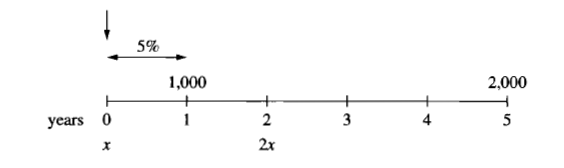
\includegraphics[scale=0.65]{picture1.PNG}

\subsection{Équation de valeur avec une période inconnue}
\label{sec:Équation valeur et période inconnue}

Pour isoler \textit{t}, on doit utilisés les logarithmes. Il existe une méthode pour faire une approximation de \textit{t}, la \emph{method of equated time}. On pose au numérateur, la valeur du paiement multiplier par son \textit{t} et au dénominateur on utilise la somme des paiements. 
\\Ex:
\\Séquence des paiements :
\\ 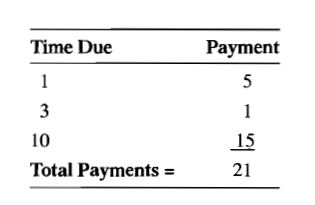
\includegraphics[scale=0.60]{picture2.PNG} 
\begin{align*}
\overline{t} = \frac{1 * 5 + 3 * 1 + 10 * 15}{(5 + 1 + 15)}
\end{align*}

\subsection{Équation de valeur avec un taux d'intérêt inconnu}
\label{sec:Équation de valeur et i inconnu}

Isoler \textit{i} algébriquement si possible, sinon utiliser la calculatrice \ref{sec:sioler i}.

%% ----- chapitre 3 -------

\chapter{Annuité}
\label{chap:annuité}

\section{Notion préliminaire}
\label{sec:Notion préliminaire}

Rappel sur les sommations : $ \sum_0^{n} = $(premier terme)$* \frac{1 - (ratio)^{\# \, terme}}{(1 - ratio)} $. Il est plus efficace de le connaitre sous forme de mots que sous la forme algébrique usuelle: $ \frac{a - ar^n}{1 - r} $.
\subsection{Truc mnémotechnique pour les annuitées}
\label{sec:astuce annuité}

Pour ne pas mélanger les dénominateurs des annuités, \textit{i} pour annuité {\large \textbf{i}}mmédiate et {\large \textit{d}} pour annuité \textbf{d}ue.

\section{Annuité immédiate et annuité due}
\label{sec:annuité immédiate et due}

\subsection{Annuité immédiate actualisée}


Une annuité immédiate actualisée ($a_{\annuity{n}i}$) est une série de paiement actualisée en fin de période. La valeur présente d'une annuité se représente comme suit :
\begin{equation}
PV = v + v^2 + v^3 + ... + v^n
\end{equation}
Donc,
\begin{equation}
PV = \frac{v(1 - v^n)}{1 - v}
\end{equation}
On se souvient qu'à la section \ref{sec:taux escompte} que $ 1 - v = d = iv $, donc si on fait une substitution,
\begin{equation}
a_{\annuity{n}i} = \frac{1 - v^n}{i}
\end{equation}

\subsection{Annuité immédiate accumulée}


Une annuité immédiate accumulée ($s_{\annuity{n}i}$) est une série de paiement accumulée en fin de période. La valeur accumulée d'une annuité se représente comme suit :
\begin{equation}
s_{\annuity{n}i} = 1 + (1 +i) + ... + (1+i)^{n-1}
\end{equation}
Donc,
\begin{equation}
s_{\annuity{n}i} = \frac{[1 - (1+i)^n]}{1-(1+i)} \Rightarrow \frac{(1+i)^n - 1}{i}
\end{equation}
On peut voir la relation suivante entre $s_{\annuity{n}i}$ et $a_{\annuity{n}i}$ ;
\begin{equation}
s_{\annuity{n}i} = (1 + i)^n a_{\annuity{n}i} = (1 + i)^n (\frac{1-v^n}{i}) = \frac{(1+i)^n - 1}{i}
\end{equation}

\subsection{Annuité due actualisée}


Une annuité due actualisée ($\ddot{a}_{\annuity{n}i}$) est une série de paiement actualisée en début de période. La valeur actualisée de cette annuité peut se représenter comme suit :
\begin{equation}
\ddot{a}_{\annuity{n}}i = 1 + v + v^2 + ... + v^{n-1} = \frac{1 - v^n}{1 - v} = \frac{1 - v^n}{d}
\end{equation}

\subsubsection{Relation entre a et $\ddot{a}$}
\label{Relation 3.1}

On peut voir rapidement la relation suivante $\ddot{a}_{\annuity{n}i} = (1+i)a_{\annuity{n}i}$.
De plus, on peut voir que 
\begin{equation}
\ddot{a}_{\annuity{n}i} = 1 + a_{\annuity{n - 1}i}
\end{equation}

\subsection{Annuité due accumulée}

Une annuité due accumulée ($\ddot{s}_{\annuity{n}i}$) est une série de paiement accumulée en début de période. La valeur accumulée de cette annuité peut se représenter comme suit :
\begin{equation}
\ddot{s}_{\annuity{n}}i = (1+i)^n + (1+i)^{n-1} + ... + (1+i) = \frac{(1+i)[1-(1+i)^n]}{1 - (1+i)} = \frac{(1+i)^n - 1}{d}
\end{equation}

\subsubsection{Relation entre s et $\ddot{s}$}
\label{Relation 3.2}

On peut voir rapidement la relation suivante $\ddot{s}_{\annuity{n}i} = (1+i)s_{\annuity{n}i}$.
De plus, on peut voir que 
\begin{equation}
{s}_{\annuity{n}i} = s_{\annuity{n + 1}i} - 1
\end{equation}

\section{Erreur à éviter avec s et $\ddot{s}$}

On peut facilement se tromper entre annuité due et annuité immédiate, ainsi que dans la valeur de l'indice n. Le document explique et démontre certaines de ces erreurs \footnote{p. 116-118}.
Afin de les éviter, voici deux astuces :
\begin{enumerate}
\item Est-ce que le dernier dépôt est fait au moment que l'on calcule l'annuité ?
Si oui, alors on utilise s, sinon on utilise $\ddot{s}$.
\item Combien de dépôt sont effectués ? Alors la fonction d'accumulation seras de n termes, sans égard à la position de ces dépôts.
\end{enumerate}

\paragraph{Note : la calculatrice possède une fonction \textit{Begin} qui permet de faire directement le calcul d'une annuité due \ref{Begin}. (sinon on peut utiliser les relations \ref{Relation 3.1} et \ref{Relation 3.2})} 

\section{Rente différé}
\label{différé}

Une rente peut-être différé, autrement dit, elle débute dans x années à partir de 0. La notation est la suivante : $ \indiceGauche{x}{\vert} a_{\annuity{n}i} $. Cette notation permet de \emph{créé} une annuité de longueur n + x à laquelle on retire une annuité de longueur x. Comme ceci,
\begin{equation}
\indiceGauche{x}{\vert} a_{\annuity{n + x}i} = a_{\annuity{n}i} - a_{\annuity{x}i}
\end{equation}
On peut aussi actualisé (ou accumulé) l'annuité sur x périodes. 
Pour une accumulation, on fait la même chose mais avec $s_{\annuity{n}i}$.

\section{Astuce sur les annuités}
\label{Astuce annuités}

Voici une méthode pour rapidement calculer les annuités en bloc avec des paiements comme ceci:
\\
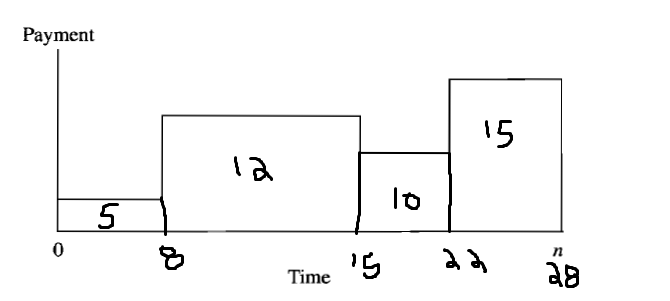
\includegraphics[scale=0.55]{picture3.PNG}.
\\La technique consiste à partir de n (ici 28), et remonter jusqu'au différent changement. On soustrait/additionne la différence le paiement de l'annuité et de la suivante.
\begin{equation}
15*a_{\annuity{28}i} - 5 * a_{\annuity{22}i} + 2 * a_{\annuity{15}i} - 7 * a_{\annuity{8}i}**
\end{equation}
** La différence entre 12 et 5.
Pour une accumulation, on fait l'inverse. On débute par la première séquence de paiement.
\begin{equation}
5*s_{\annuity{28}i} + 7 * s_{\annuity{20}i} - 2 * s_{\annuity{13}i} + 5 * s_{\annuity{6}i}
\end{equation}

\section{Perpétuité}
\label{Perpétuité}

Il s'agit d'une annuité avec $ n \rightarrow \infty$. Le concept de perpétuité ne s'applique pas à la fonction  d'accumulation, la fonction est divergente.
\begin{equation}
a_{\annuity{\infty}i} = \frac{1}{i} \quad \text{et} \quad \ddot{a}_{\annuity{\infty}i} = \frac{1}{d}
\end{equation}

\section{Astuce pour annuité de kn terme sur n terme }
\label{Astuce annuité}

Certains problèmes dans les examens peuvent être résolus par le ratio $\frac{a_{\annuity{2n}i}}{a_{\annuity{n}i}}$. Le ratio donne ceci :
\begin{equation}
\frac{a_{\annuity{2n}i}}{a_{\annuity{n}i}}  = \frac{\frac{1 - v^{2n}}{i}}{\frac{1 - v^n}{i}} = \frac{1 - v^{2n}}{1 - v^n}
\end{equation}
Comme $1 - v^n $ est une différence de deux carrés, on peut le factorisé par $(1 + v^n) (1 - v^n)$.
\begin{equation}
\label{équation chap3-1}
\frac{a_{\annuity{2n}i}}{a_{\annuity{n}i}}  = \frac{(1 + v^n) (1 - v^n)}{1 - v^n} = 1+v^n
\end{equation}
De plus, pour $\frac{\ddot{a}_{\annuity{2n}i}}{\ddot{a}_{\annuity{n}i}}$, le résultat est le même. Ce résultat s'applique aussi pour d'autre ratio d'annuité. Ex.: (ici, on utilise une 2e approche pour trouver la solution)
\begin{equation}
a_{\annuity{3n}i} = a_{\annuity{n}i} + v^{n}a_{\annuity{n}i} + v^{2n}a_{\annuity{n}i} = a_{\annuity{n}i}(1 + v^{n} + v^{2n})
\end{equation}
Donc,
\begin{equation}
\frac{\ddot{a}_{\annuity{3n}i}}{\ddot{a}_{\annuity{n}i}} = \frac{a_{\annuity{n}i}(1 + v^{n} + v^{2n})}{a_{\annuity{n}i}} = (1 + v^{n} + v^{2n})
\end{equation}
On peut faire le même processus pour des accumulations, soit :
\begin{equation}
\frac{s_{\annuity{2n}i}}{s_{\annuity{n}i}} = \frac{\frac{(1+ i)^{2n}}{i}}{\frac{(1+i)^{n}}{i}} = \frac{(1+i)^{2n}-1}{(1+i)^{n} -1}
\end{equation}
On fait une différence de deux carrés comme à l'équation \ref{équation chap3-1}. 
\begin{equation}
\frac{s_{\annuity{2n}i}}{s_{\annuity{n}i}}  = \frac{((1+i)^n - 1) ((1+i)^n + 1)}{1 - v^n} = (1+i)^n + 1
\end{equation}


\section{Période inconnue}
\label{période inconnue}

Dans certain cas, si \textit{n} est inconnue, le dernier paiement peut ne pas être un entier. Il faut alors, selon le problème ; 
\begin{enumerate}
\item avoir un dernier paiement plus élevé (pour la période $\lfloor n \rfloor$) ;
\item avoir un paiement plus petit (pour la période $\lceil n \rceil$;
\item faire un dernier paiement final à la période n exacte.
\end{enumerate}

\section{Taux inconnu}
\label{taux inconnu}

Si on connait \textit{n}, la valeur actualisée ou la valeur accumulée et la valeur du paiement, on utilise la calculatrice et la fonction TVM pour isoler \textit{i}. (voir annexe \ref{sec:sioler i})

\section{Taux intérêt variable}
\label{Taux intérêt variable et annuité}

Le taux d'intérêt peut varier dans le temps (ou être en fonction d'une force d'intérêt), il devient essentiel de bien associer les taux avec les bons paiements. voici deux exemples \footnote{ASM 10 \ieme édition p.170} :
\\
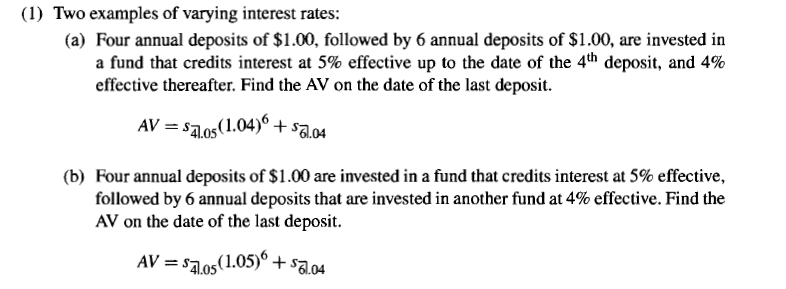
\includegraphics[scale=0.80]{picture4.PNG}


%% ---------------- Chapitre 4

\chapter{Annuités 2.0}
\label{Annuités 2.0}

\section{Annuité avec \emph{off-payments}}
\label{Annuité off-payments 1.0}
Il s'agit d'annuité ou la fréquence des paiements est plus ou moins fréquente que le taux d'intérêt. 
\\Exemple 4.1\label{Exemple4.1}: Un taux annuel de 5 \% pour une annuité de paiement au 2 ans. La fréquence de paiement est donc moins fréquente que le taux d'intérêt. Deux méthodes d'approche peuvent être utilisées pour résoudre le problème.

\begin{enumerate}
\item On peut utiliser le taux d'intérêt pour l'équivalent de la période de paiement. Si on réutilise l'exemple \ref{Exemple4.1}, le 5 \% est exprimé pour une période de 1 an. Le taux équivalent 2 ans est donc, 
\begin{equation}
(1.05)^2 = (1 + j) \qquad j = 10.25 \%
\end{equation}
\item On peut aussi utiliser le taux d'intérêt du problème, soit 5 \%.
\end{enumerate}
La première méthode est la plus efficace pour arriver à des résultats numériques. La deuxième méthode est efficace pour sortir les valeurs symboliques.

\section{Annuité avec \emph{off-payments} 2.0}
\label{Annuité off-payments 2.0}

Ici, on voit la deuxième méthode de résolution des annuités avec \emph{off-payments}.

\subsection{Paiement moins fréquent que la période d'intérêt (\emph{Fission method}}
\label{fission method}

On place les paiements sur une ligne du temps et on trouve la somme géométrique de ceux-ci. On veut avoir des séquences répétitives de paiement durant toute la durée totale de l'annuité. (voir p. 175-177)

\subsection{Paiement plus fréquent que la période d'intérêt (\emph{Fussion method}}
\label{Fussion method}

Voici la notation : 
\begin{equation}
a_{\annuity{n}i}^{(m)} = \frac{1-v^n}{i^{(m)}}
\end{equation}
On peut aussi trouver la relation suivante,
\begin{equation}
a_{\annuity{n}i}^{(m)} = \frac{1}{i^{(m)}}a_{\annuity{n}i}
\end{equation}
Ce qui revient à fusionner les paiements compris dans une période, sous une seule période. Ex. : 12 paiements mensuels avec un taux nominal annuel $\textit{i}^{(12)} $de 12\%. On veut \emph{créé} une annuité équivalente de paiement R de 1 an, qui revient à une annuité de 12 paiements mensuels pour le taux nominal 12 \%. Alors, $ R = \frac{i}{i^{(12)}}$, comme il s'agit d'une accumulation on peut dire que $ R = s_{\annuity{1}^{(12)}i}$.
Démonstration, 
\begin{equation}
s_{\annuity{1}^{(12)}i} = \frac{(1+i)^1 - 1}{i^{(12)}} \Rightarrow \frac{i}{i^{(12)}}
\end{equation}
De cette relation, on peut trouver ceci;
\begin{equation}
a_{\annuity{n}i}^{(m)} = \frac{1 - v^{n}}{i^{(m)}} = \frac{i}{i^{(m)}} a_{\annuity{n}i} \Rightarrow s_{\annuity{1}i}^{(12)} a_{\annuity{n}i}
\end{equation}
On fait le même relation pour une accumulation,
\begin{equation}
s_{\annuity{n}i}^{(m)} = \frac{1 - v^{n}}{i^{(m)}} = \frac{i}{i^{(m)}} s_{\annuity{n}i} \Rightarrow s_{\annuity{1}i}^{(12)} s_{\annuity{n}i}
\end{equation}
Pour une annuité due,
\begin{equation}
\ddot{a}_{\annuity{n}i}^{(m)} = \frac{1 - v^{n}}{d^{(m)}} = \frac{i}{d^{(m)}} a_{\annuity{n}i} \Rightarrow \ddot{s}_{\annuity{1}i}^{(12)} a_{\annuity{n}i}
\end{equation}
Même processus pour une accumulation.
Pour des annuités à perpétuité, on voit rapidement que $v^n$ lorsque $n\longrightarrow \infty$ va donner 0, alors les équations pour une annuité due et immédiate seront ;
\begin{equation}
\label{equ:chap4}
a_{\annuity{\infty}i} = \frac{1}{i^{(m)}}, \quad \ddot{a}_{\annuity{\infty}i} = \frac{1}{d^{(m)}}
\end{equation}

\subsubsection{Relation importante de l'équation \ref{equ:chap4} }
\label{sub:sub:relation imporante}

La seule différence entre une perpétuité due et une perpétuité immédiate est la suivante :
\begin{equation}
\ddot{a}_{\annuity{\infty}i} - a_{\annuity{\infty}i} = \frac{1}{d^{(m)}} - \frac{1}{i^{(m)}} = \frac{1}{m}
\end{equation}

Note : Comme il est illustré dans la section \emph{4C} du document p. 181, il est important de rassembler les paiements à l'intérieur de la même période. 
\\Ex.:
\\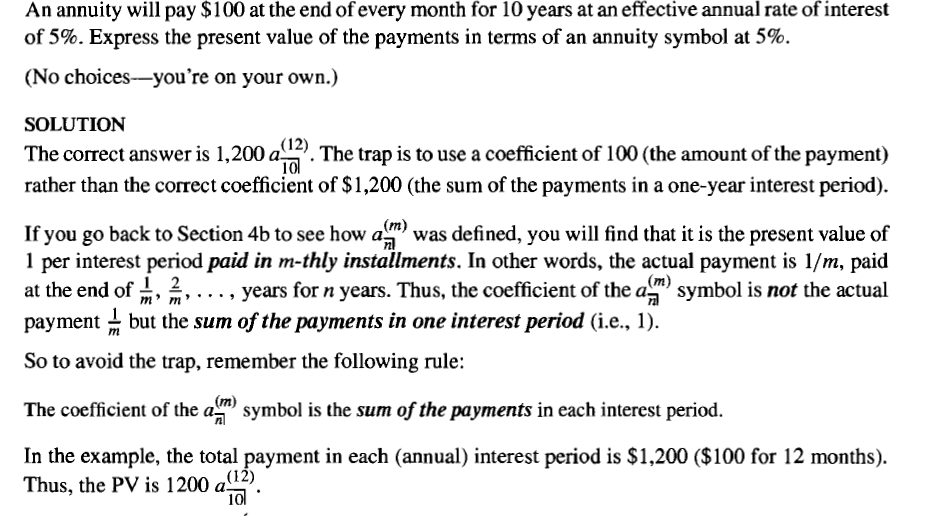
\includegraphics[scale=0.55]{picture5.PNG}

\section{Annuité avec paiement continu}
\label{Annuité continu}

Il s'agit d'annuité ou la fréquence m des paiements $\longrightarrow \infty$. Si on regarde la limite d'une annuité due ou immédiate on note que $\lim\limits_{m \to \infty } i^{(m)} = \lim\limits_{m \to \infty } d^{(m)} = \delta$. Donc, il n'y a pas de différence entre annuité due et immédiate. On se retrouve alors avec ceci;
\begin{equation}
\lim\limits_{m \to \infty } a_{\annuity{n}i}^{(m)} = \frac{1 - v^n}{\delta} = \overline{a}_{\annuity{n}i} \quad *
\end{equation}
* Rappel équation \ref{chap1:équation delta} : $\delta = \ln(1+i)$.
\\La relation suivante peut-être établi par la suite :  
\begin{equation}
\overline{a}_{\annuity{n}i} = \frac{i}{\delta}a_{\annuity{n}i}
\end{equation}  

\subsubsection{Annuité continu et intégrale}
\label{sub:sub:continu et integrale}
\begin{equation}
\overline{a}_{\annuity{n}i} = \int_{0}^{n} v^{t} \, \mathrm{d}t = \frac{v^{n} - 1}{\ln v}
\end{equation}
Comme $\ln v = \ln(1+i)^-1 = - \ln(1+i) = - \delta $.
\begin{equation}
\frac{v^{n} - 1}{\ln v} = \frac{1 - v^{n}}{\delta} = \overline{a}_{\annuity{n}i}
\end{equation}

\section{Astuce avec double annuité due}
\label{Astuce double dot}

Si on exprime $ \ddot{a}_{\annuity{n}i} / \ddot{a}_{\annuity{p}i} $ on obtient $ a_{\annuity{n}i} / a_{\annuity{p}i} $.
On peut le démontrer :
\begin{equation}
\frac{\ddot{a}_{\annuity{n}i}}{\ddot{a}_{\annuity{p}i} } = \frac{\frac{1 -v^n}{d}}{\frac{1 -v^p}{d}} = \frac{1 -v^n}{1-v^p} = \frac{a_{\annuity{n}i}}{a_{\annuity{p}i}}
\end{equation}
On peut appliquer cette relation à d'autre annuité :
\begin{equation}
\frac{\ddot{a}_{\annuity{n}i}^{(m)}}{\ddot{a}_{\annuity{p}i}^{(m)}} = \frac{\ddot{a}_{\annuity{n}i}}{\ddot{a}_{\annuity{p}i}} = \frac{a_{\annuity{n}i}}{a_{\annuity{p}i}} = \frac{a_{\annuity{n}i}^{(m)}}{a_{\annuity{p}i}^{(m)}}
\end{equation}
On peut aussi établir les relations suivante si $ p = \frac{1}{2n} $ à partir de \ref{Astuce annuité} :
\begin{equation}
\frac{\ddot{a}_{\annuity{2n}i}^{(m)}}{\ddot{a}_{\annuity{n}i}^{(m)}} = \frac{\ddot{a}_{\annuity{2n}i}}{\ddot{a}_{\annuity{n}i}} = \frac{a_{\annuity{2n}i}}{a_{\annuity{n}i}} = \frac{a_{\annuity{2n}i}^{(m)}}{a_{\annuity{n}i}^{(m)}} = 1 + v^n
\end{equation}
À noter, le taux d'intérêt doit être le même pour les deux annuités.

\section{Accumulation et taux variable}
\label{trap alert accumulation et taux variable}

Si un problème d'accumulation utilise un taux variable, il est important de se rapeller la définition de la fonction d'accumulation avec intérêt variable \ref{sec:sub:taux interet variable}. Si on veut connaitre l'accumulation de n paiements après \textit{t} années, on obtient :
\begin{equation}
s_{\annuity{t}i} = \frac{a(t)}{a(t)} + \frac{a(t)}{a(t-1)} + \frac{a(t)}{a(t-2)} + ... + \frac{a(t)}{a(1)}
\end{equation}
Si on fait une mise en évidence on obtient :
\begin{equation}
s_{\annuity{t}i} = a(t)[\frac{1}{a(t)} + \frac{1}{a(t-1)} + \frac{1}{a(t-2)} + ... + \frac{1}{a(1)}]
\end{equation}

\section{Annuité avec paiement variable}
\label{sec:Annuité paiement variable}

Une annuité avec paiement suivant une progression arithmétique \footnote{ASM p 209}. 
\\Exemple:
\begin{align*}
A & = 5v + 8v^2 + 11v^3 + ... + 29 v^9 + 32v^{10}
\end{align*}
Il existe une astuce algébrique pour résoudre une équation polynomiale de degré k. On multiplie l'équation par (1+i), et on soustrait l'équation A à l'équation Ai :
\begin{align*}
(1+i)A & = 5 + 8v + 11v^2 + ... + 29 v^8 + 32v^9 \\
iA & = 5 + 8v + 11v^2 + ... + 29 v^8 + 32v^9 - (5v + 8v^2 + 11v^3 + ... + 29 v^9 + 32v^{10}) \\
Donc, \quad iA & = 5 + 3(v +v^2 + v^3 + ...+v^9) - 32v^{10}
\end{align*}
On voit que $ 3(v +v^2 + v^3 + ...+v^9) = 3a_{\annuity{9}i} $.
\begin{align*}
A & = \frac{5 + 3a_{\annuity{9}i} -32v^{10}}{i}
\end{align*}
Pour une forme générale de cette \emph{astuce} :
\begin{equation}
\label{eq:chap4:1}
A = Pa_{\annuity{n}i} + Q \frac{a_{\annuity{n}i} - nv^{n}}{i} 
\end{equation}
Il s'agit d'une série de paiement dont le premier paiement est plus grand que 1 et de progression artihmétique plus grande que 1.
\\Où P est la valeur du premier terme et Q la valeur de la progression arithmétique (dans l'exemple, P = 5, Q= 3). On trouve aussi les équations suivantes :
\begin{equation}
\label{eq:chap4:2}
\ddot{A} = (1+i)A = P\ddot{a}_{\annuity{n}i} + Q \frac{a_{\annuity{n}i} - nv^{n}}{d}
\end{equation}
\begin{equation}
\label{eq:chap4:3}
S = Ps_{\annuity{n}i} + Q \frac{s_{\annuity{n}i} - n}{i}
\end{equation}
\begin{equation}
\label{eq:chap4:4}
\ddot{S} = P\ddot{s}_{\annuity{n}i} + Q \frac{s_{\annuity{n}i} - n}{d}
\end{equation}
On peut facilement trouver les équations \ref{eq:chap4:2}(High life), \ref{eq:chap4:3} et \ref{eq:chap4:4} à partir de l'équation \ref{eq:chap4:1} et de la relation $ (1+i)a_{\annuity{n}i} = \ddot{a}_{\annuity{n}i} $ (ou avec une accumulation).

\subsection{Annuité à progression arithmétique (\emph{Increasing annuity})}
\label{Sub:Chap4:increasing}

Il s'agit d'un cas particulier de l'équation \ref{eq:chap4:1} où P = Q = 1.
\begin{equation}
(Ia)_{\annuity{n}i} = (1)a_{\annuity{n}i} + (1) \frac{a_{\annuity{n}i} - nv^{n}}{i} 
\end{equation}
Que l'on peut exprimer comme suit pour annuité immédiate et annuité due:
\begin{align*}
(Ia)_{\annuity{n}i} & = a_{\annuity{n}i} + \frac{ia_{\annuity{n}i} + a_{\annuity{n}i} - nv^{n}}{i}\\
& = \frac{(1+i)a_{\annuity{n}i} - nv^n}{i} 
\end{align*}
\begin{equation}
(Ia)_{\annuity{n}i} = \frac{\ddot{a}_{\annuity{n}i} - nv^n}{i} \quad \text{et} \quad (I\ddot{a})_{\annuity{n}i} = \frac{\ddot{a}_{\annuity{n}i} - nv^n}{d}
\end{equation}
Pour obtenir une accumulation, on multiplie l'équation par $(1+i)^n $ et par $(1+i)^{n+1}$ pour obtenir $(I\ddot{s})_{\annuity{n}i} $:
\begin{equation}
(Is)_{\annuity{n}i} = \frac{\ddot{s}_{\annuity{n}i} - n}{i} \quad \text{et} \quad (I\ddot{s})_{\annuity{n}i} = \frac{\ddot{s}_{\annuity{n}i} - n}{d} 
\end{equation}
Si on fait une substitution de $ \ddot{s}_{\annuity{n}i}$ par $s_{\annuity{n+1}i} -1 $, on obtient :
\begin{equation}
(Is)_{\annuity{n}i} = \frac{s_{\annuity{n+1}i} - (n+1)}{i}
\end{equation}
Voir annexe \ref{annuité et TI-30XS} pour utilisation de la calculatrice TI-30XS avec les annuités.

\subsection{Annuité à décroissance arithmétique (\emph{Decreasing annuity})}
\label{Sub:Chap4:decreasing}

Il s'agit d'un autre cas particulier de l'équation \ref{eq:chap4:1} où P = n et  Q = -1.
\begin{equation}
(Da)_{\annuity{n}i} = na_{\annuity{n}i} - \frac{a_{\annuity{n}i} - nv^{n}}{i} 
\end{equation}
Que l'on peut exprimer comme suit pour immédiate et due:
\begin{equation}
 (Da)_{\annuity{n}i} = \frac{n - a_{\annuity{n}i}}{i} \quad \text{et} \quad  (D\ddot{a})_{\annuity{n}i} = \frac{n -a_{\annuity{n}i}}{d}
\end{equation}
Pour obtenir une accumulation, on multiplie l'équation par $(1+i)^n $ et par $(1+i)^{n+1}$ pour obtenir $(D\ddot{s})_{\annuity{n}i} $:
\begin{equation}
(Ds)_{\annuity{n}i} = \frac{n(1+i)^n - s_{\annuity{n}i}}{i} \quad \text{et} \quad  (D\ddot{s})_{\annuity{n}i} = \frac{n(1+i)^n -a_{\annuity{n}i}}{d} 
\end{equation}
Voir annexe \ref{annuité et TI-30XS} pour utilisation de la calculatrice TI-30XS avec les annuités.

\subsubsection{Astuce pour les annuités à progression arithmétique}
Une méthode simple pour résoudre des problèmes avec des paiements variables est la suivante \footnote{ASM p. 212} :
\begin{enumerate}
\item Trouver la différence entre les paiements(k) et écrire une (Ia)/(Is) ou une (Da)/(Ds) avec paiement de k
\item Ajouter ou soustraire la valeur manquante sous forme d'annuité (actualisation ou accumulation) normale
\end{enumerate}
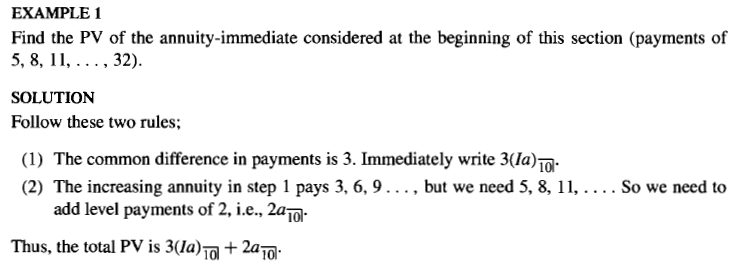
\includegraphics[scale=0.61]{picture6.PNG}

\subsection{Annuité à perpétuité croissante}
\label{Increasing perpetuities}

On a les équations suivantes :
\begin{equation}
(Ia)_{\annuity{\infty}i} = \frac{1}{id} = \frac{1}{i} + \frac{1}{i^2} \quad \text{et} \quad (I\ddot{a})_{\annuity{\infty}i} = \frac{1}{d^2}
\end{equation}
Pour une forme générale P et Q à partir de l'équation \ref{eq:chap4:1} :
\begin{align*}
PV = \lim\limits_{n \to \infty}( Pa_{\annuity{n}i} + Q \frac{a_{\annuity{n}i} - nv^{n}}{i})
\end{align*}
\begin{equation}
= \frac{P}{i} + \frac{Q}{i^2}
\end{equation}
\subsection{Annuité croissante suivie par une perpétuité constante}

La valeur présente d'une annuité croissante de \textit{n} termes suivie d'une annuité à perpétuité de paiement n\$ se représente comme ceci :
\begin{align*}
PV & = (Ia)_{\annuity{n}i} + v^{n}(\frac{n}{i}) \\
 & = \frac{\ddot{a}_{\annuity{n}i} - nv^{n} + nv^{n}}{i}
\end{align*}
\begin{equation}
PV = \frac{\ddot{a}_{\annuity{n}i}}{i}
\end{equation}

\section{Notation suplémentaire sur annuité}
\begin{enumerate}
\item \textit{I} signifie que le taux annuel de paiement augmente 1 fois par année. Ex.: $(Ia)_{\annuity{n}i}$
\begin{equation}
(Ia)_{\annuity{n}i} = \frac{\ddot{a}_{\annuity{n}i} - nv^n}{i}
\end{equation}
Voir section \ref{Sub:Chap4:increasing} et \ref{Sub:Chap4:decreasing} pour toute les équations.
\item $I^{(m)}$ signifie que le taux annuel de paiement augmente m fois par an. Donc, paiement de $\frac{1}{m}$ dans la première 1/m période, suivie de $\frac{2}{m}$ dans la seconde 1/m période. 
\\Ex.: $(I^{(6)}a)_{\annuity{n}i}$ le paiement augmente à chaque 6 mois.
\begin{equation}
(Ia)_{\annuity{n}i}^{(m)} = \frac{\ddot{a}_{\annuity{n}i} - nv^n}{i^{(m)}}
\end{equation}
Voir section \ref{Sub:Chap4:increasing} et \ref{Sub:Chap4:decreasing} pour toute les équations.
\item \textit{a} signifie que le paiement est annuellement.
\item $ a^{(m)}$ signifie que le paiement est fait m fois par an.
\item $(Ia)_{\annuity{n}i}^{(m)}$ signifie qu'il y a progression des paiements à chaque année \textit{(I)}, mais qu'il y a m paiements de i/m par année (i est croissant/décroissant).
\item \emph{The double m annuity} $(I^{(m)}a)_{\annuity{n}i}^{(m)}$ signifie que le taux annuel de paiement augmente à tout les 1/m et qu'il y a m paiements par période. Donc, on se retrouve avec des paiements de $\frac{1}{m^2}, \frac{2}{m^2},...,\frac{mn}{m^2}$.
Le livre comporte un exemple appliqué de cette annuité, problème \# 46 p. 230.
\begin{equation}
(I^{(m)}a)_{\annuity{n}i}^{(m)} = \frac{\ddot{a}_{\annuity{n}i}^{(m)} - nv^n}{i^{(m)}}
\end{equation}
Voir section \ref{Sub:Chap4:increasing} et \ref{Sub:Chap4:decreasing} pour toute les équations.
\item $(I^{(\infty)}a)_{\annuity{n}^{(\infty)}i} = (\overline{I}\overline{a})_{\annuity{n}i}$ Il s'agit de la \emph{ double m annuity} ou $ m\longrightarrow \infty $ (paiement continu).
\begin{equation}
\label{eq:chap4:double continuos annuity}
(\overline{I}\overline{a})_{\annuity{n}i} = \frac{\overline{a}_{\annuity{n}i} - nv^n}{\delta}
\end{equation}
Voir section \ref{Sub:Chap4:increasing} et \ref{Sub:Chap4:decreasing} pour toute les équations.
\end{enumerate}

\section{Annuité à progression géométrique}
\label{annuité géométrique}

Annuité avec une croissance géométrique, exemple une annuité indexé avec le taux d'inflation. Il est donc facile de faire une somme des termes et de trouver la récurence. Pour un rappel sur les sommations voir \ref{sec:Notion préliminaire}.
En général, pour une annuité avec un premier paiement de 1 \$, on peut utiliser la forme général suivante \footnote{Voir ASM p. 244-245}:
\begin{equation}
PV = \frac{1 - (\frac{1+k}{1+i})^n}{i-k}
\end{equation}
On peut aussi exprimer la somme géométrique sous une \emph{annuité normale} avec un taux \textit{i} modifier, soit \textit{i'}.
\begin{enumerate}
\item Mettre en évidence les termes récurent de la sommation
\item On exprime le nouveau taux \emph{i'} par $\frac{1 + \text{taux croissance des paiements}}{1+i}$
\end{enumerate}
En général , le taux \emph{i'} peut-être exprimer par : $\frac{i - k}{1+k}$ où k est le taux de variation des paiements. Si $k>i$ alors, on utilise $\frac{k-i}{1+i}$.

\section{Annuité à taux variable continu}
\label{sec:taux variable continu}

\subsubsection{$\overline{a}_{\annuity{n}i}$}
Correspond à une annuité continu avec un taux constant durant la période t. Le taux d'intérêt varie selon la fonction $f(t)$ où $f(t) =1$, voici une représentation graphique:
\\
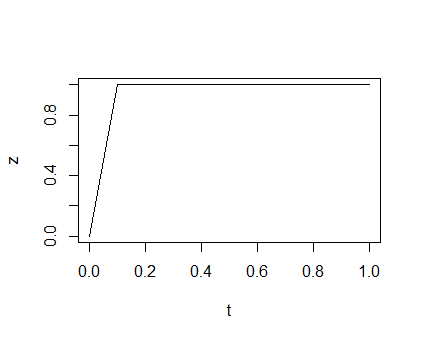
\includegraphics[scale=0.60]{picture8.png}
\\
Pour trouver la valeur accumulé à \textit{n} de $\overline{a}_{\annuity{n}i}$ on fait l'intégrale :
\begin{align*}
\overline{a}_{\annuity{n}i} = \int_{0}^{n} v^{t} \, \mathrm{d}t = \frac{1 - v^{n}}{\delta}
\end{align*}
Ce qui correspond à la formule trouver dans la section \ref{sub:sub:continu et integrale}.

\subsubsection{$(\overline{I}\overline{a})_{\annuity{n}i}$}
Correspond à une annuité continu avec un taux continu de croissance. Le taux d'intérêt varie selon la fonction $f(t)$ où $f(t) =t$, voici une représentation graphique:
\\
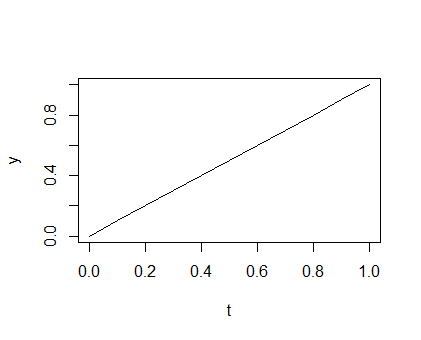
\includegraphics[scale=0.60]{picture7.png} 
\\
Pour trouver le valeur accumulé à \textit{n} de $(\overline{I}\overline{a})_{\annuity{n}i}$ on fait l'intégrale :
\begin{equation}
(\overline{I}\overline{a})_{\annuity{n}i} = \int_{0}^{n} tv^{t} \, \mathrm{d}t = \frac{\overline{a}_{\annuity{n}i} - nv^{n}}{\delta}
\end{equation}
Ce qui correspond à l'équation \ref{eq:chap4:double continuos annuity}.
\\
Pour une annuité avec un taux d'intérêt variable en continu, il faut une $f(t)$ où $f(t)$ varie dans le temps mais que $v^t$ soit constant. Pour trouver la valeur accumulé à n on fait l'intégrale de $f(t)$ :
\begin{equation}
PV = \int_{0}^{n} v^{t}f(t) \, \mathrm{d}t
\end{equation}
Dans le cas ou $v^t$ n'est pas constant et varie selon une force d'intérêt $\delta$ , alors on se retrouve avec ceci :
\begin{equation}
PV = \int_{0}^{n} f(t)e^{-\int_{0}^{t} \delta_r \mathrm{d}r} \, \mathrm{d}t
\end{equation}

\section{Annuité Palindromic}
\label{sec:palindromic}

Il s'agit d'une annuité symétrique, ex: 1,2,3,4,5,4,3,2,1. On peut résoudre une t'elle annuité algébriquement ou utilisé un raccourci.
\begin{enumerate}
\item Algébriquement : On fait une annuité croissante additionner avec une annuité décroissante différé.
\item On peut aussi représenter cette série de paiement comme une série d'annuité différé. Pour avoir la valeur présente on fait donc une annuité de cette série d'annuité.  
\end{enumerate}
Exemple de la seconde méthode. On a la séquence de paiement suivante :\\
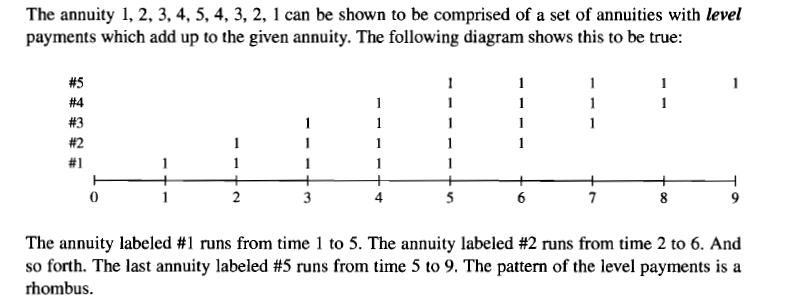
\includegraphics[scale=0.59]{picture9.PNG}\\
On voit qu'au temps 0, 1, 2, 3 et 4 on débute une annuité de 5 périodes. On peut donc résumer cette série de paiement ainsi :
\begin{equation}
PV= a_{\annuity{n}i} \ddot{a}_{\annuity{n}i}
\end{equation}
La première annuité représente les paiements de 1\$ et la seconde annuité représente la séquence des annuités au temps 0, 1, 2, 3 et 4. Voici une représentation graphique :
\\
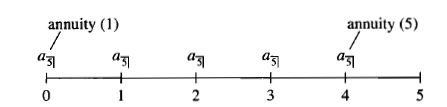
\includegraphics[scale=0.65]{picture10.PNG}

\section{L'astuce 0\% pour les réponses sous forme symbolique}
\label{sec:astuce0}

Il s'agit d'un test pour évaluer des réponses exprimés sous leurs formes symboliques. On utilise un taux d'intérêt à 0\% pour éliminer les réponses impossibles. On commence par évaluer la série de paiement avec un taux 0\% et ensuite on évalue les formes algébriques donnée au même taux. Valeur des annuités avec un taux 0\% :
\begin{align*}
a_{\annuity{n}i} & = n  = \ddot{a}_{\annuity{n}i}\\
s_{\annuity{n}i} & = n  = \ddot{s}_{\annuity{n}i}\\
(Ia)_{\annuity{n}i} & = \frac{n(n+1)}{2} = (Is)_{\annuity{n}i} \\
(1+i)^n & = 1 \\
V^n & = 1 \\
i = d & =\delta = 0\\ 
\end{align*}
\\
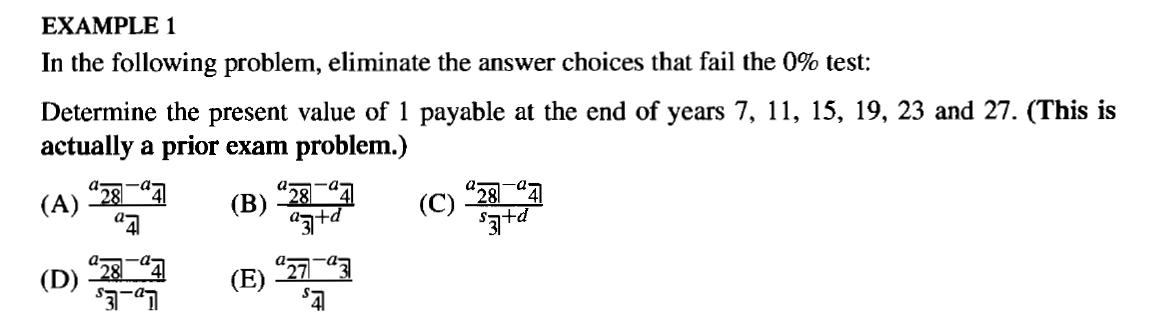
\includegraphics[scale=0.60]{picture11.PNG} 
La VP de la série de paiement = 6 ($a_{\annuity{6}i}  = 6$). Ensuite, on fait de même avec les 5 réponses.
\\
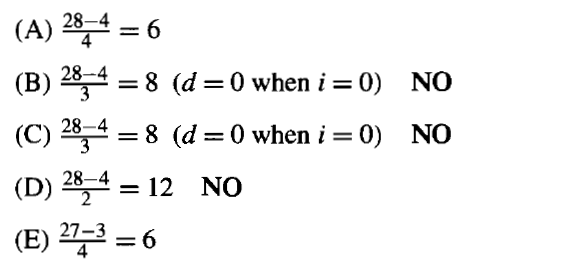
\includegraphics[scale=0.55]{picture12.PNG}
\\
**Note: Fonctionne seulement si \textit{i} est inconu. 


%% ---------------- Chapitre 5

\chapter{Taux de rendement (\emph{Yield rates})}
\label{chp:yield}

\subsection{Flux de trésorie actualisé}
\label{sub:flux trésorie}

\subsubsection{Valeur actualisé nette (VAN)}
\label{sub:sub:VAN}

Il s'agit de la VP des flux de trésories entrant moins la VP des flux de trésorie sortant. On choisit la VAN la plus élevée lorsqu'on à des investissement mutuellement exclusif. On ne choisit pas une série de paiement avec une VAN négative. 
\begin{equation}
VAN = \sum A_tv^t - \sum L_tV^t = \sum(A_t-L_t)v^t
\end{equation}
Où $A_t$ est flux de trésorie entrant et $L_t$ représente un flux de trésorie sortant.
\\ On peut représenter la VAN comme une fonction de \textit{i}, $P(i)$.
\begin{align*}
P(i) = -L_0 + A_1v^1 + A_2v^2
\end{align*}

\subsubsection{Taux de rendement interne (TRI) (\emph{internal rate of return-IRR})}
\label{IRR}

Il s'agit du taux d'intérêt \textit{i} qui permet d'avoir la VAN à 0\$, soit $P(i) = 0$. Il y au au maximum autant de solution possible (réel, irréel ou négative) que de changement de signe dans la série de paiement.
\\ 
Il existe deux solutions pour résoudre $P(i)$ :
\begin{enumerate}
\item On teste les valeurs de \emph{i} donné en réponse (essaie et erreur)
\item On utilise la calculatrice (voir ...)
\end{enumerate}
Mise en garde : Le TRI ne donne pas toujours des solutions possibles. On peut se retrouver avec un \textit{i} très grand ou seulement des valeurs négatives.

\section{Taux de réinvestissement}
\label{sec:Taux reinvestissement}

Certain problème présente des réinvestissement des intérêts dans un autre compte. On peut souvent regrouper les problèmes (en général) en 2 types :
\begin{enumerate}
\item Un investissement initial de x \$ et on reinvestis les intérêts. On peut donc résoudre le problème comme suit : $AV= x\$ (1 + i*s_{\annuity{n}i'})$.
\item Une série d'investissement constant sur n période de x \$ et on reinvestis les intérêts. On obtient donc : $AV = x\$ (n  + i*(Is)_{\annuity{n}i'})$.
\end{enumerate}

\section{La mesure d'intérêt d'un fonds}
\label{sec:mesure intérêt d'un fonds}

Méthode pour approximer le taux de rendement d'un fonds avec 3 informations :
\begin{enumerate}
\item Montant au départ (A)
\item Montant à la fin (B)
\item L'intérêt gagné dans le fonds(en \$)
\end{enumerate}
\begin{align*}
A(1+i) + \sum C_{t}(1+i)^{1-t} & = B, \text{ où $C_t$ est un cashflow} \\
A(1+i) + \sum C_{t}(1+(1-t)i) & = B, \text{Avec un taux d'intérêt simple}\\
i = \frac{B - A - C}{A + \sum C_{t}(1 - t)} & , \text{ où C est un $\sum C_t$} \\
\end{align*}
Si on fait une interprétation du numérateur; le montant à la fin de la période = montant au début de la période + dépôt net (dépôts - retrait) + intérêt. 
\\$B = A + C +I$
\\$I= B- A - C$
Alors on obtient,
\begin{equation}
\label{eq:chap5:equation I}
i = \frac{I}{A + \sum C_{t}(1 - t)}
\end{equation}
On peut supposer que le montant net des dépôts se produit à t = 1 / 2, alors,
\begin{align*}
i = \frac{I}{A + \frac{C}{2}}
\end{align*}
Pour exprimer l'expression en fonction de A, B et des intérêts gagné on exprime $ C = B -A -I$,
\begin{equation}
i = \frac{2I}{A + B - I}
\end{equation}

\section{Taux d'intérêt à dollar pondéré et temps pondéré}
\label{Dollar pondéré et temps pondéré}

\subsection{Dollar pondéré}

Définition : Le taux d'intérêt en dollar pondéré correspond à l'estimation en taux d'intérêt simple du taux de rendement. L'estimation en taux d'intérêt simple est calculé avec la fonction linéaire vue à la section \ref{note:chap1}. Cette méthode consiste à trouver le taux d'intérêt simple tel que tous les dépôts accumulés à la fin de l'année moins tous les retraits accumulés à la fin de l'année donne la balance du fonds à la fin de l'année. Pour calculer \textit{i} on utilise l'équation \ref{eq:chap5:equation I}.

\subsection{Temps pondéré}
Pour trouver le rendement en temps pondéré on utilise \footnote{Notes de cours de mathématiques financières chapitre 5 p. 26} :
\begin{equation}
i = \prod_{k=1}^{n+1} \frac{F_k}{F_{k-1} + C_{k-1}} - 1, \quad \text{où $F_k$ est le solde du compte au temps k}
\end{equation}
Il est plus simple de démontrer avec un exemple du livre :
\\
\includegraphics[scale=0.60]{picture13.PNG} 

\section{Méthodes du portefeuille et de l'année d'investissement}
\label{sec:portefeuille}
Les deux méthodes peuvent aussi être utilisé ensemble, exemple : les trois premières années sont MAI et par la suite on utilise la méthode du portefeuille.

\subsubsection{Méthode du portefeuille}
Cette méthode attribue le même \% de rendement à tous les membres du portefeuille sans égard à la date d'entrée et le montant.

\subsubsection{Méthode de l'année d'investissement (MAI)}
Cette méthode tient compte de l'année d'entrée dans le fonds et attribue des rendements différents selon cette date. Donc, un investissement qui débute en 2006 n'auras pas la même séquence d'intérêt les années suivantes qu'un investissement débutant en 2007 dans le même fonds.


%% ---------------- Chapitre 6

\chapter{Tableaux d'amortissement et fonds d'amortissement}

\section{Amortissement d'un prêt}
Note : J'ai principalement utilisé les notes de mathématiques financières pour cette section voir document \href{https://drive.google.com/open?id=0B6kXivc6X9LITmdBVFVWSDAxeE0}{mathématiques financières} dans le Google Drive.

Lorsqu'on fait une paiement de k\$ sur un prêt une partie sert à payer les intérêts et la différence (k- intérêt) est un paiement sur le capital. Le solde du prêt (\emph{outstanding balance}) diminue et le montant des intérêts sur la prochaine période diminue aussi. La somme des intérêts payé plus la somme de capital payé = t * k.
\textbf{Notation pour la section:}
\begin{itemize}
\item L : le montant du prêt (à \textit{t} = 0) = $OB_0$
\item $OB_j$, j=1, 2, ..., \textit{n} : Balance du prêt (capital)
\item $I_j$, j=1, 2, ..., \textit{n} : intérêts payés pour la période j
\item $PR_j$, j=1, 2, ..., \textit{n} : principal remboursé pour la période j
\item \textit{n} : le nombre de paiements périodiques 
\item \textit{i} : le taux d'intérêt par période
\item $K_j$, j=1, 2, ..., \textit{n} : les montants des paiements
\end{itemize}

\subsection{Méthode générale d'amortissement}
\label{sec:amortissement général}

\begin{equation}
L = \sum_{j=1}^{n}K_{j}v^{j}
\end{equation}

\subsection{Forme rétrospective de la balance du prêt au temps \textit{t}}
\label{sec:rétrospective}

On cherche à trouver la balance de capital en regardant les transactions antérieurs à \textit{t}.

\begin{equation}
OB_t = OB_0(1+i)^{t} - \sum_{j=1}^{t}K_j(1+i)^{t-j}
\end{equation}
Pour obtenir le principal et l'intérêt payé au temps \textit{t}:
\begin{equation}
\label{eq:chap6:principal et intérêt}
PR_t = OB_{t-1}- OB_t, \quad PR_t = K_t - I_t, \qquad I_t = iOB_{t-1} 
\end{equation}

\subsection{Forme prospective de la balance du prêt au temps \textit{t}}
\label{sec:prospective}

On cherche à trouver la balance du capital en regardant les prochaines transactions à venir (\textit{looking forwar}). La forme général :
\begin{equation}
OB_t = \sum_{j=1}^{n-t}K_{t+j}v^{j}
\end{equation}
Pour le calcul du principal et de l'intérêt on utilise les équations du point \ref{eq:chap6:principal et intérêt}.

\subsection{Amortissement d'un prêt avec paiement égaux}
\label{sec:amortissement prêt}

Lorsqu'on fait des paiements égaux, on note que le montant de principal payé suit une progression géométrique avec un ratio (1+\textit{i}). Le montant des paiements $K = \frac{L}{a_{\annuity{n}i}}$. On se retrouve avec les \emph{équations} suivante :
\begin{align*}
OB_0 & = Ka_{\annuity{n}i} \\
OB_t & = OB_0(1+i)^t - Ks_{\annuity{t}i}, \quad \text{\textbf{Méthode rétrospective}} \\
OB_t & = Ka_{\annuity{n-t}i}, \quad \text{\textbf{Méthode prospective}} \\
I_t & = iOB_{t-1}= Kia_{\annuity{n-t+1}i} = K[1- v^{n-t + 1}] \\
PR_t & = Kv^{n-t+1} \\
I_{total} & = K \sum_{t=1}^{n}[1 -v^{n-t + 1}] = K[n -a_{\annuity{n}i}] \\
\end{align*}
On peut utilisé la calculatrice pour faire une table d'amortissement \ref{ann:chap:amortissement}.

\section{Fonds d'amortissement}
\label{sec:sinking fund}
Il s'agit d'un fonds servant à accumuler la capital nécessaire pour le paiement d'un prêt en totalité (un prêt où seulement les intérêts sont payé par période).
\begin{align*}
\text{Valeur du placement dans le fonds} & = \frac{\text{Prêt}}{s_{\annuity{n}j}} \\
\text{Valeur du paiement total par période} & = \text{Prêt}*i + \frac{\text{Prêt}}{s_{\annuity{n}j}}
\end{align*}
Le taux d'intérêt sur le prêt est souvent différent du taux d'intérêt sur le placement $ i \neq j$.

\section{Balance du prêt, intérêts payés et principal payé avec un fonds d'amortissement}
\label{sec: OB, PR, I from sinking fund}

Le solde d'intérêt net d'un fonds d'amortissement correspond au montant d'intérêt payé moins le montant d'intérêt gagné dans le fonds. On voit plus clairement le phénomène lorsque le taux d'intérêts du prêt est égal au taux d'intérêt du fonds, $ i = j $. Donc, le montant des intérêts décroit dans le temps.
\\
\\
Pour la balance du prêt, elle correspond au montant net du capital. Il s'agit du montant du prêt moins le montant dans le fonds. Autrement dit, si demain l'emprunteur utilise le fonds pour payer le prêt combien lui manque-t-il. Donc, le montant du capital restant est décroissant dans le temps.
\\
\\
Le montant de principal payé correspond au montant de capital payé sur le prêt. Trois méthodes sont utilisées pour déterminer le montant de principal payé :
\begin{enumerate}
\item L'intérêt gagné dans le fonds d'amortissement durant la période \textit{t} plus le dépôt fait à la fin de la période.
\item Le montant accumulé jusqu'à la période \textit{t} moins le montant accumulé jusqu'à la période \textit{t - 1 }.
\item On peut aussi trouver le capital payé en retirant le montant des intérêt payé sur le montant payé sur le prêt.
\end{enumerate}

\section{Série de paiement variable}
\label{sec:sinking fund paiement variable}

Un prêt peut être payé par des paiements variable, il faut alors construire un tableau d'amortissement et utilisé les équations \ref{eq:chap6:principal et intérêt}. Cette méthode peut entrainer une capitalisation des intérêts si le paiements est inférieur au paiements d'intérêt à faire. On sait déjà que $OB_n = 0 \quad \text{et que} \quad PR_n = L $.  Exemple de tableau :
\\
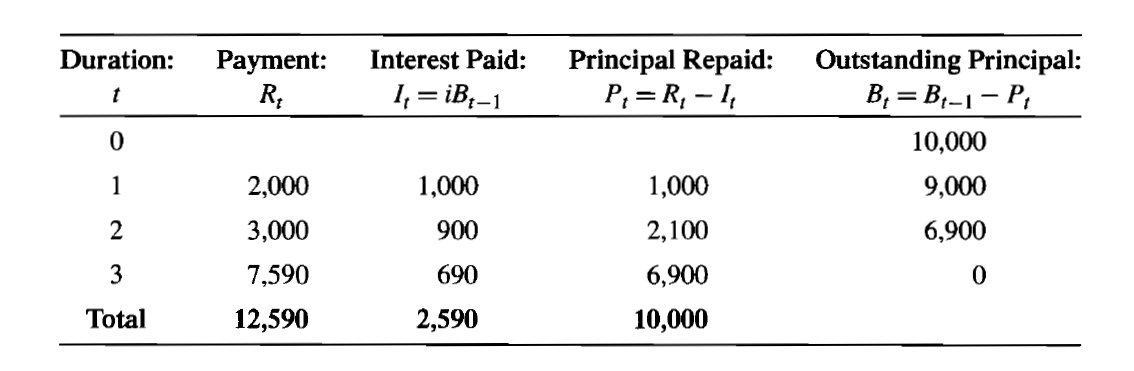
\includegraphics[scale=0.45]{picture14.PNG}
\\
En général on peut utilisé cette relation entre deux paiements succesif de principal :
\begin{equation}
PR_t = (1 + i)P_{t-1} + (K_t - K_{t-1})
\end{equation}

\subsection{Paiement égaux de principal}
\label{equal principal payments}

Il s'agit d'un cas particulier des série de paiement variable. Il s'agit de faire des paiements égaux de principal plus les intérêts à payé.  Il y a donc une décroissance des paiements car le capital diminue d'un montant constant.



%% ---------------- Chapitre 7

\chapter{Les obligations}
\label{Chap:obligations}

Terminologie des obligations et notations:
\begin{enumerate}
\item Prix de l'obligation (\textit{P})
\item Valeur nominale : montant du prêt (\textit{par/face value}) (\textit{F})
\item Coupons : paiement par période des intérêts (\textit{C})
\item Taux de coupon : taux d'intérêt par période sur la valeur nominale, valeur fixe et déterminé au départ (\textit{r})
\item Nombre de période : échéance (\textit{n})
\item Valeur de rachat (à maturité)(\textit{redemption value})
\item Taux de coupon modifié : le taux de coupon appliqué à \textit{c} pour déterminé le montant du coupon $ g = \frac{Fr}{C}$
\item Taux d'intérêt par période : le taux d'intérêt \textit{i} pour lequel \textit{P} = la VP de la série de paiement. Valeur qui change dans le temps (\textit{i})
\end{enumerate}
Habituellement, au Canada et aux États-Unis, le versement des coupons se fait par période de 6 mois en taux nominale. Le prix d'achat d'une obligation varie selon les taux sur le marché et le taux de coupon.
\\
\\\textbf{Note importante :} Si la valeur de rachat n'est pas spécifiée, il faut assumer que la valeur nominale = la valeur de rachat \footnote{ASM p.378}. 
\pagebreak

\subsection{Formule des obligations}
\label{sub:sec:formules obligtions}

\begin{equation}
P = Fr a_{\annuity{n}i} + Cv^{n}
\end{equation}
\begin{equation}
P = Cg a_{\annuity{n}i} + Cv^{n}
\end{equation}
À partir de la définition algébrique d'une annuité : $ a_{\annuity{n}i} = \frac{1 -v ^{n}}{i} \Longrightarrow 1- ia_{\annuity{n}i} $
\begin{align*}
P & = Cg a_{\annuity{n}i} + Cv^{n} \\
& = Cg a_{\annuity{n}i} + C(1- ia_{\annuity{n}i})
\end{align*}
alors, 
\begin{equation}
P = C + (Fr - Ci)a_{\annuity{n}i}
\end{equation}
\begin{equation}
P = C + (Cg - Ci)a_{\annuity{n}i} \Longrightarrow P = C( 1 + (g - i)a_{\annuity{n}i})
\end{equation}
La loi de Makeham est surtout utilisé dans un contexte de série d'obligations.
\begin{align*}
P & = Cg a_{\annuity{n}i} + Cv^{n} \\
P & = Cg (\frac{1 - v^{n}}{i}) + Cv^{n} \\
P & =  \frac{g}{i}(C-Cv^{n}) + Cv^{n}
\end{align*}
Si on pose $k = Cv^{n}$,
\begin{equation}
P =  K + \frac{g}{i}(C-K)
\end{equation}

\section{Premium et discount}
\label{sec:premium et discount}

Premium : Valeur marchande > valeur de rachat (g > i), amortissement du premium (capital).
\\Discount : Valeur marchande < valeur de rachat (g < i), capitalisation des intérêts.
\\Donc, pour calculer les premiums et avoir une idée de la valeur de marché, il faut utiliser l'équation :
\begin{equation}
P = C + (Cg - Ci)a_{\annuity{n}i}
\end{equation}
On peut calculer le \textit{book value} (balance du capital) de la même façon qu'un prêt \ref{sec:amortissement prêt}. L'amortissement du premium se fait en progression géométrique :
\begin{equation}
P_t = (Fr - Ci)v^{n-t+1}, \quad \text{où} \quad P_t = (Cg - Ci)v^{n-t+1}
\end{equation}
Où $P_t$ correspond au montant de premium payé.
\\La capitalisation des intérêts pour un discount peut se calculer avec :
\begin{equation}
P_t = (Ci -Cg)v^{n-t+1}
\end{equation}

\section{Prix d'obligation entre deux coupons}
\label{sec:price between}

On considére le prix d'une obligation pour une fraction de période entre deux coupons.  Deux prix pour une obligation entre deux dates sont utilisés :
\begin{enumerate}
\item Le prix réellement payé lors de l'achat (\emph{settlement date})
\item Le prix affiché dans la presse financière soit le prix excluant la valeur du coupon non versé (intérêts accumulés)
\end{enumerate}

\subsection{Prix réel d'achat}
\label{sub:sec:prix réel}

On suppose que le dernier coupon payé se fait au temps \textit{t} et que l'obligation se vend au temps $ t + k $, où $ 0 \leq k \leq 1 $.
\begin{equation}
B_{t+k} = (1+i)^{k}B_{t}
\end{equation}
Où exprimer comme la valeur présente du prochain coupon :
\begin{equation}
B_{t+k} = V^{1-k}(B_{t+1} + Fr)
\end{equation}

\subsection{Prix affiché dans la presse financière}
\label{sub:sec:presse financiere}

On retire la valeur accumulé d'intérêt du coupon.
\begin{equation}
B_{t+k} - kFr = B_{t}(1+i)^{k} - kFr
\end{equation}

\subsection{Représentation graphique du prix des obligations}
\label{sub:sec:graphique obligations}

Obligation avec un premium:
\\
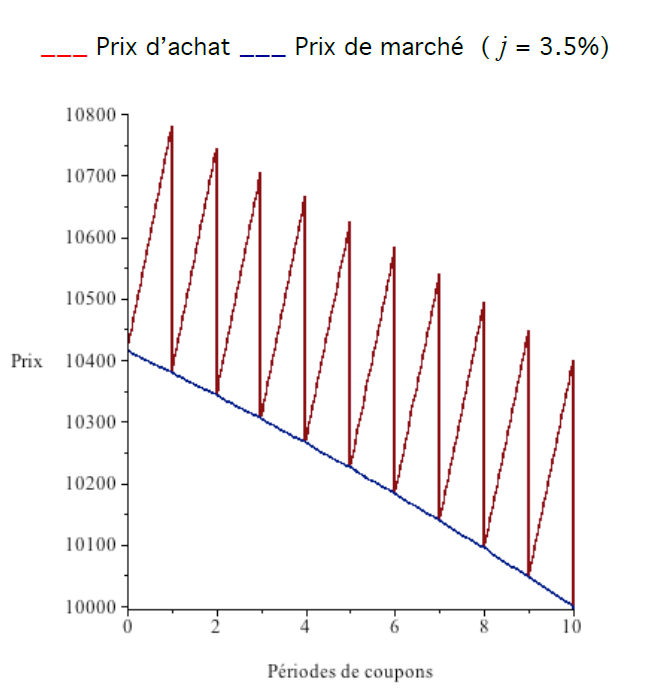
\includegraphics[scale=0.40]{picture15.PNG} 

Obligation à parité:
\\
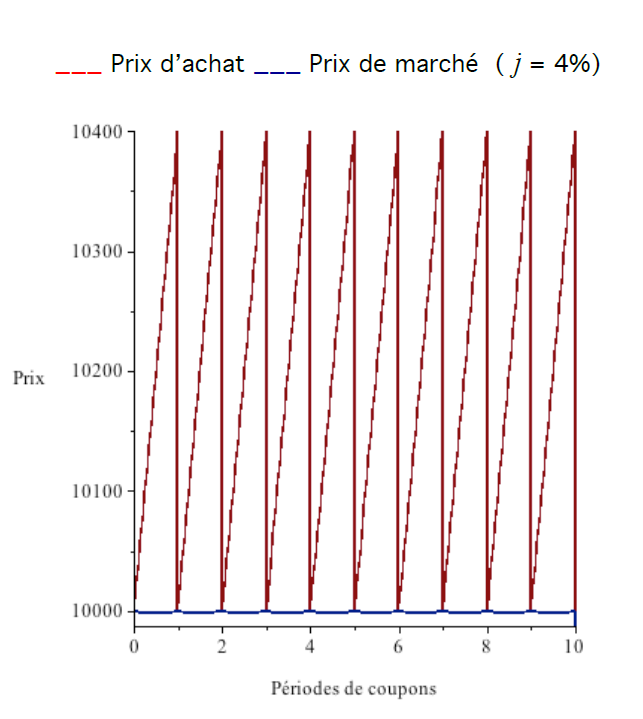
\includegraphics[scale=0.40]{picture16.PNG}

Obligation avec discount:
\\
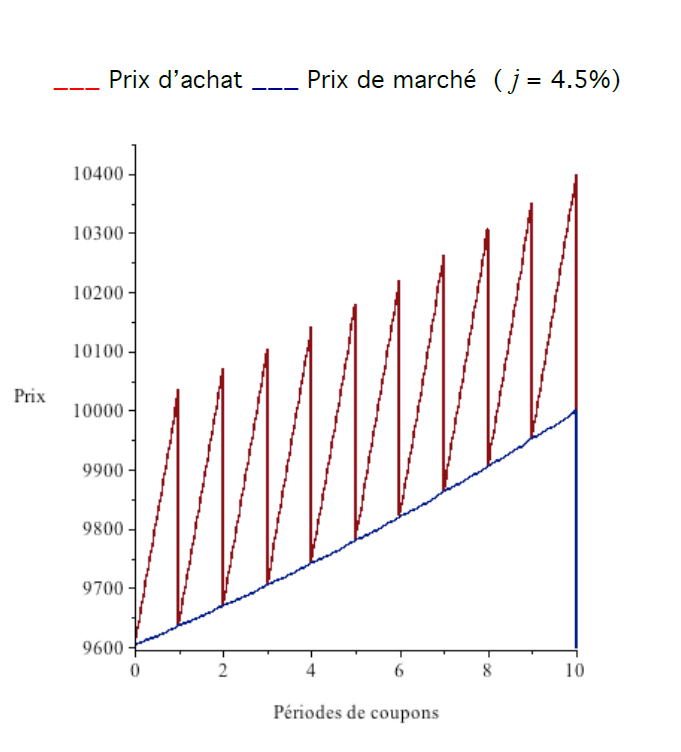
\includegraphics[scale=0.40]{picture17.PNG} 

\subsection{Nombre de jours}
\label{sex:nombre de jours}

Technique pour compter le nombre de jours entre 2 coupons. 

\subsubsection{\emph{Actual/actual method}}

Cette technique est utilisé pour les obligations du gouvernement. Le nombre actuel de jours est utulisé au numérateur et k au dénominateur. Il s'agit d'un ratio sur maximum 365 jours. Afin de calculé le nombre de jours, la calculatrice possède une fonction, voir le livret d'instruction \href{https://drive.google.com/open?id=0B6kXivc6X9LIMXI4T1QtcTFQNzA}{page 91}.

\subsubsection{\emph{30/360 method}}

Cette technique est utilisé pour les obligations d'entreprise et de municipalité. Avec cette méthode chaque mois est considéré avoir \textbf{exactement 30 jours}. Donc, il y a 360 jours dans l'année.

\section{Obligation rachetable}
\label{sec:callable bonds}

Permet à l'émeteur de racheter les oblications à la valeur de rachat. Habituellement, une date est fixé quelques années après l'émission (\emph{call date}). Cette option influence le taux de rendement de l'obligation. S'il y a un premium (g > i), le pire rendement de l'obligation sera la date de rachat de l'obligation (\textit{call date}). S'il y un discount (g < i), le pire rendement sera la date la plus éloigné.
\\ Astuce mnémotechnique :
Pour le taux de rendement d'une obligation \textbf{P}remium, \emph{the \textbf{E}arliest date is the \textbf{W}orst}, appeler le principe \textbf{PEW}.
\subsubsection{Application général}
Dans certaine situation, plusieurs montants et date de rachat peuvent être possible. Pour avoir une méthode général d'application, le rendement minimum se calcul avec le prix le plus pas possible selon les valeurs et dates de rachat.


%% ---------------- Chapitre 8

\chapter{Instruments financiers}
\label{chap:financial instruments}

Section sur la théorie de GRF I, type d'actifs financier. Je n'ai pas traiter la section sur les autres types d'actifs financiers (fonds commun de placement, bons du Trésors...) mais voici de la documentation du cours de GRF sur la matière vue sur le sujet : \href{https://drive.google.com/open?id=0B6kXivc6X9LIV09sWEZlLWNtdmc}{chapitre 1}, \href{https://drive.google.com/open?id=0B6kXivc6X9LIdVRwUGRhd0xBR1k}{chapitre 2} et \href{https://drive.google.com/open?id=0B6kXivc6X9LIXzRxSlVsdktMN1E}{chapitre 14}

\section{Obligations, actions et actions privilégier}
\label{sec:actifs financiers}
Les principales sources de financement des entreprises sont : la dette (obligation) et les actions. Il existe d'autres types d'investissements plus \emph{spécifique} des obligations, tel que les \emph{junk bonds} et les \emph{zero-coupon bond}. Les \emph{junk bonds} sont des obligations plus risqués que les obligations gouvernementales. Elle servent principalement de financement lors de prise de contrôle. Les  \emph{zero-coupon bonds} sont des obligations sans coupon. Il peut s'agir d'un paiement complet du principal et intérêt à la fin du terme ou d'une obligation \emph{STRIPS}. Une obligation \emph{STRIPS} signifie que chaque coupons ainsi que la valeur de rachat sont transigé comme des obligations  \emph{zero-coupon bond} indépendante.
Cette image résume très bien les notions générale des trois types d'actifs financiers \footnote{ASM p. 427} :
\\
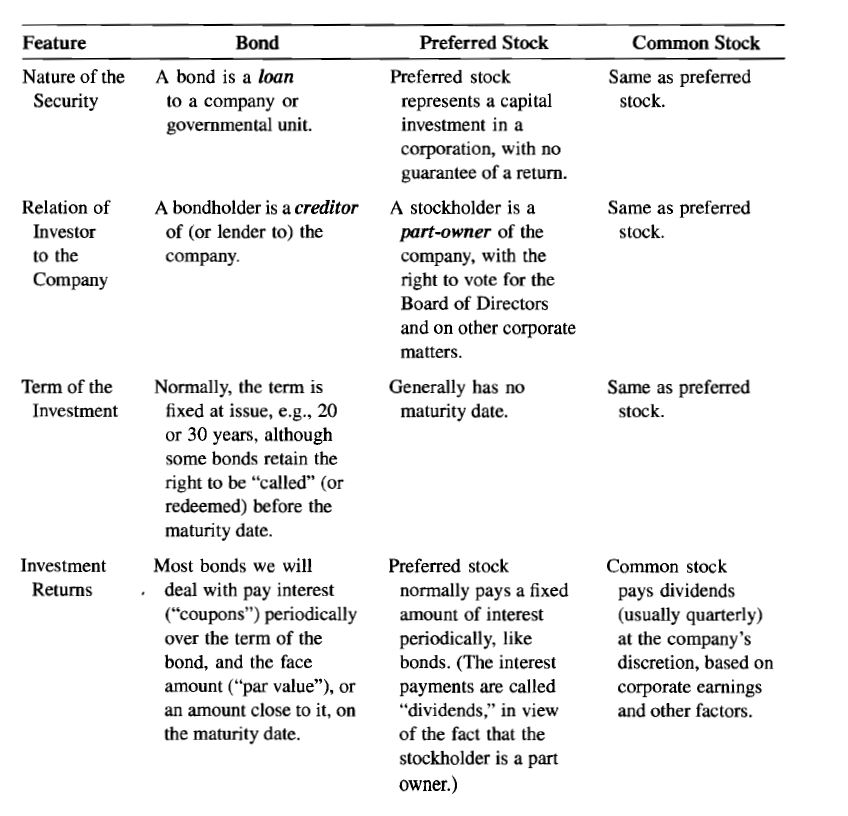
\includegraphics[scale=0.5]{picture18.PNG} 
\\
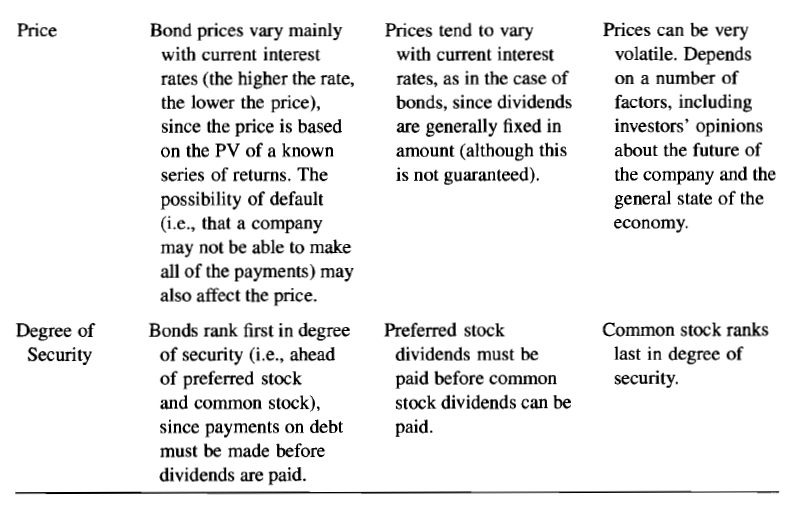
\includegraphics[scale=0.5]{picture19.PNG}
\\
\section{Prix des instruments}
\label{sec:price share stock}
Pour déterminer le prix des actions privilégier ou les obligations à perpétuité :
\begin{equation}
P = \frac{Fr}{i}
\end{equation}
Pour déterminer le prix des actions ordinaires, on utilise le modèle d'actualisation des dividendes: (où D est le montant de dividende et (1+k) est la croissance du dividende s'il y à lieu)
\begin{equation}
P = Dv + D(1+k)v^2 + D(1+k)^2vç3 + ... = \frac{D}{i - k}
\end{equation}

%% ---------------- Chapitre 9

\chapter{Analyse financière avancée}
\label{cha:advanced financial analysis}

\section{Inflation}
\label{sec:inflation}

Le taux d'intérêt réel est le taux d'intéret en prenant compte de l'inflation. Souvent appeler le \emph{market rate}.
\begin{equation}
1 + i' = \frac{1+i}{1+r}
\end{equation}
Exprimer en mots : $( 1 + \textit{real rate})= \frac{(1 + \textit{market rate})}{(1 + \textit{inflation rate})}$
\begin{equation}
i'=\frac{i-r}{1+r}
\end{equation}
Pour des taux d'intérêts petit, on peut dire avec une précision appréciable que $i' = i -r $

\section{Taux forward, taux au comptant et taux de rendement}
\label{sec:spot, forward et yield}

La courbe des taux de rendements est généralement croissante positive. Ce phénomène s'explique en grande parti avec la théorie de la structure à terme. L'incertitude du temps créé une pression sur les taux de rendement demandé pour des échéanciers plus long. 

\section{Taux au comptant \emph{Spot rate}}
\label{sec:spot rate}

Taux de rendement moyen applicable pour des obligations zero-coupon (taux des obligations sans coupon). Correspond aussi à la moyenne géométrique des taux forward.
\begin{equation}
S_n = [(1+f_1)(1+f_2)...(1+f_n)]^{1/n} - 1
\end{equation}

\section{Taux forward}

Il s'agit du taux anticipé pour une période dans le futur,  $f_t$ (noter que t = t+1). Donc, le taux forward pour t = 3 s'exprime $ f_2 $.

\begin{equation}
1+f_t = \frac{a(t+1)}{a(t)} = \frac{(1+s_{t+1})^{t+1}}{(1+s_{t})^{t}}
\end{equation}

\section{Duration}
\label{duration}

La duration correspond à la durée moyenne des flux monétaires. On pondère le flux avec ca période. On utilise le même principe  que celui de la section \ref{sec:Équation valeur et période inconnue}.
\begin{equation}
D = \frac{\sum CF_{t}*(t)} {\sum CF_{t}}
\end{equation}

\section{Duration de Macaulay}
\label{sec:duration macaulay}

La duration de Macaulay correspond à la durée moyenne des flux monétaires actualisés.
\begin{equation}
MacD = \frac{\sum (V^{t}*CF_{t})*(t)}{\sum V^{t}*CF_{t}}
\end{equation}
On peut aussi exprimer la duration comme la dérivée du prix par rapport à $\delta$ sur le prix. 
\begin{equation}
\frac{\dfrac{d}{d\delta}P(i)}{P(i)} 
\end{equation}

\subsection{Autre relation importante}

Si on a un n-year bond avec des coupons annuel avec $P = F = C$, on peut démontrer que la MacD donne $\ddot{a}_{\annuity{n}i}$:
\begin{align*}
MacD = & \frac{r(v+2v^2+...+nv^n) + nv^v}{\text{prix obligation}} \\
= & r(Ia)_{\annuity{n}i} + nv^n \\
= & r \frac{\ddot{a}_{\annuity{n}i} - nv^n}{i} + nv^n
\end{align*}
Comme $r=i$,
\begin{equation}
MacD = \ddot{a}_{\annuity{n}i}
\end{equation}

\section{Duration modifiée}
\label{sec:modified duration}

La duration modifié correspond à la sensibilité du prix lors d'un changement de taux d'intérêt.
\begin{equation}
ModD = \frac{\sum (V^{t+1}*CF_{t})*(t)}{\sum V^{t}*CF_{t}} \Leftrightarrow v [\frac{\sum (V^{t}*CF_{t})*(t)}{\sum V^{t}*CF_{t}}]
\end{equation}
\begin{equation}
ModD = -\frac{P'(i)}{P(i)} = -\frac{\frac{d}{di}P(i)}{P(i)} \Rightarrow v MacD 
\end{equation}

Il s'agit autrement dit, de la variation de la duration, appeler parfois la volatilité.

Pour approximer le changement de prix :
\begin{equation}
\Delta P = - (ModD)(P)(\Delta i)
\end{equation}
Où $\Delta i$ correspond à la variation du taux d'intérêt (positive si augmentation et négative si diminution).

\section{Duration d'un portefeuille}
\label{sec:duration portefeuille}

\begin{equation}
MacD = \frac{\sum P_t*(MacD)_t}{\sum P_t}
\end{equation}
Où $P_t$ est le prix de l'obligation t.

\section{Convexité}
\label{Convexité}

Soit la dérivée seconde du prix. Exprimer en pourcentage du prix.
\begin{align*}
\text{Convexité} = \frac{\frac{d^2}{di^2} P}{P}
\end{align*}
\begin{equation}
\text{Convexité} = \frac{\sum_{t} t * (t+1) * V^{t+2} * CF_{t}}{P(i)}
\end{equation}
Pour faire une approximation de la variation du prix :
\begin{equation}
\Delta P \approx P(i) *[-(\Delta i)*(ModD) + \frac{1}{2}*(\Delta i)^2 *(\text{Convexité})]
\end{equation}

\section{Immunisation de Redington}
\label{sec:immunisation de Redington}

L'immunisation de Redington assure une protection contre des petites variation du taux d'intérêt. Les trois conditions à l'immunisation de Redington :
\begin{enumerate}
\item La valeur présente des actifs financiers = la valeur présente des engagement financiers
\item La duration des actifs financiers = la duration des engagements financiers
\item La convexité des actifs financiers > convexité des engagements financiers
\end{enumerate}

On peut résumé ainsi ces trois conditions (A pour Actifs et L pour Liabilities):
\begin{enumerate}
\item $P_A = P_L$ 
\item $P'_A = P'_L$
\item $P"_A > P"_L$
\end{enumerate}

\section{Immunisation complète}
\label{sec:immunisation complète}

L'immunisation complète assure une protection contre toutes les variations du taux d'intérêt. Les trois conditions à l'immunisation complète :
\begin{enumerate}
\item La valeur présente des actifs financiers = la valeur présente des engagement financiers
\item La duration des actifs financiers = la duration des engagements financiers
\item Il y a un flux monétaire entrant (des actifs financiers) avant un flux monétaire sortant pour un engagement financier
\end{enumerate}

\section{Appariement}
\label{sec:appariement}

On \textit{attache} un actifs financiers pour chaque flux de trésorie sortant. Il s'agit de poser une quantité pour chaque flux de trésorie et de résoudre le système d'équation.

\section{Duration et convexité éffective}
\label{sec:duration effective}

Certain flux monétaire peuvent être influencé par les teux d'intérêt, ex. une obligation rachetable. Le prix n'est donc pas toujours différentiable. On utilise alors la duration éffective et la convexité effective.

\begin{equation}
EffD = \frac{P(i-h)-P(i+h)}{2*h*P(i)}
\end{equation}
\begin{equation}
EffC = \frac{P(i+h)-P(i-h)- 2*P(i)}{h^{2}*P(i)}
\end{equation}



%% ---------------- Chapitre 10

\chapter{Produit dérivé}
\label{cha:produit dérivé}

*J'ai rajouter des liens vers \href{http://www.investopedia.com/?o=40186&l=dir&qsrc=999&qo=investopediaSiteSearch}{\textit{Investopedia}} pour une descriptions vidéos des concepts.
\\Un \href{http://www.investopedia.com/terms/d/derivative.asp?o=40186&l=dir&qsrc=1&qo=serpSearchTopBox&ap=investopedia.com}{produit dérivé} est un contrat qui fluctue en fonction du taux ou du prix d'un produit sous-jacent. Le réglement s'effectue à une date future. Utilité des produits dérivé :
\begin{enumerate}
\item Gestion du risque (\href{http://www.investopedia.com/terms/h/hedge.asp?o=40186&l=dir&qsrc=1&qo=serpSearchTopBox&ap=investopedia.com}{\textit{hedging}}) : Protection contre les fluctuation future du produit, d'un bien, d'un produits financiers, ou autre.
\item Spéculation financière sur un bien, un titre ou autre.
\item Réduction des coûts de transaction.
\item Taxes et impôts, stratégie financière fiscale pour diminuer son imposition.
\end{enumerate}

\section{Developpement et utilisation des produits dérivés}
\label{sec:developpement et utilisation}

Pour une bonne descriptions de cette section voir le document \footnote{ASM p. 494-495}.

\section{Vente et achat de produits financier}
\label{sec:vente achat}

Lors d'une vente on doit payé des frais de commission. Il a deux prix lors de la vente le \href{http://www.investopedia.com/terms/b/bid-and-asked.asp?o=40186&l=dir&qsrc=999&qo=investopediaSiteSearch}{\emph{bid price}}, le prix d'achat, et le \href{http://www.investopedia.com/terms/b/bid-and-asked.asp?o=40186&l=dir&qsrc=999&qo=investopediaSiteSearch}{\emph{ask price}}, le prix de vente. Le \emph{ask price} est plus élevée que le \emph{bid price}. Le \href{http://www.investopedia.com/terms/b/bid-askspread.asp?o=40186&l=dir&qsrc=999&qo=investopediaSiteSearch}{\emph{bid-ask price}} est la différence entre les deux prix. 

\section{\emph{Short-Selling Assets}}
\label{sec:short-selling assets}

\href{http://www.investopedia.com/terms/l/long.asp?o=40186&l=dir&qsrc=999&qo=investopediaSiteSearch&ap=investopedia.com}{\textbf{Long position (in the stock):}}  Achat \textit{réel} des actions (ou autres titres).
\\
\\ \href{http://www.investopedia.com/terms/s/short.asp?o=40186&l=dir&qsrc=999&qo=investopediaSiteSearch}{\textbf{Short position :}}  On \emph{emprunte} les actions (ou autres titres) ensuite on les vends au prix courant. À une date prédéterminé on rachète les actions au nouveau prix courant et on \textit{redonne} les actions (appeler \href{http://www.investopedia.com/terms/c/closeposition.asp?o=40186&l=dir&qsrc=999&qo=investopediaSiteSearch&ap=investopedia.com}{\emph{closing/covering the short position}}). Dans le cas ou le prix à diminuer il y a un gain. Il ne s'agit pas d'un emprunt ou on rembourse le prix de l'action mais bien de rembourser par une nouvelle action.

Pour diminuer le risque le prêteur de titre peut demander un dépôt de \emph{sécurité} appeler un \href{http://www.investopedia.com/terms/h/haircut.asp?o=40186&l=dir&qsrc=1&qo=serpSearchTopBox&ap=investopedia.com}{\emph{haircut}}. Des intérêts sont versé sur le dépôt, le taux d'intérêt est appeler \emph{short rebate} pour les actions et \emph{repo rate} pour les obligations. Dans le cas des dividendes, comme ils ne sont pas versé à aucune des deux parties (actions vendus), l'emprunteur doit payé les dividendes au prêteur. 



%% ---------------- Chapitre 11

\chapter{Contrat à terme}
\label{cha:contrat à terme}

Un \href{http://www.investopedia.com/terms/f/forwardcontract.asp?o=40186&l=dir&qsrc=999&qo=investopediaSiteSearch}{contrat à terme}, est un contrat qui lie deux parties dans la vente et l'achat d'une quantité de titre (\emph{underlying asset}). Un contrat à terme spécifié la quantité, la date d'expriation du contrat (date ou la transaction à lieu) et le prix d'achat.
\\
L'acheteur dans le contrat possède la \emph{long position}, donc de sont point de vue, il s'agit d'un \emph{long forward}. L'acheteur est gagant si le prix du titre augmente.
\\ Le vendeur dans le contrat possède la \emph{short position}, donc de sont point de vue, il s'agit d'un \emph{short forward}. Le vendeur est gagant si le prix du titre diminue.

\section{\emph{The payoff}}

Pour déterminer le \emph{payoff} :
\begin{itemize}
\item Payoff to long forward : Spot price at expiration - forward price ($S_{T} - F$)
\item Payoff to short forward : forward price - spot price at expiration ($F - S_{T}$)
\end{itemize}
* Spot price : le prix du titre  sur le marché cette journée
\\
** Forward price : Prix de vente et d'achat dans le contrat
\\
Le paiement peut aussi se faire en argent plutot qu'en transaction d'action pour éviter les frais de commission et le \emph{bid-ask spread}.



%% ---------------- Chapitre 12

\chapter{Option d'achat (\emph{Call option})}
\label{chap: call options}

Contrairement à un contrat à terme, une option d'achat offre l'option d'acheter à un prix convenu un titre. Il n'y a pas d'obligation d'achat, mais il y a obligation de vente. Une option d'achat comprend une prime.
\\ Terminologie :
\begin{enumerate}
\item Acheteur (\emph{purchaser}) : La personne qui achéte l'option d'achat. 
\\Caractéristiques : Sans obligation, \emph{purchased call} et \emph{long position}.
\item Vendeur (\emph{Writer}) : La personne qui vend l'option.
\\Caractéristiques : Obligation de vente, \emph{written call} et \emph{short position}.
\item Le prix d'exercice (\emph{strike price}) (K): Prix de vente du titre avec l'option d'achat
\item Date d'expiration (\emph{expiration date})
\end{enumerate}
Il existe deux styles d'options d'achats :
\begin{enumerate}
\item Style Européen : L'option d'achat peut seulement être utilisée au moment de la date d'expiration. Européen = Expiration
\item Style Américain : L'option d'achat peut être utilisée à tout moment. Américain = Anytime
\end{enumerate}
\begin{equation}
\label{eq:chap:12:payoff long call}
\text{\emph{Payoff} sur un \emph{purchased/long call}} = max[0, S_T - K]
\end{equation}
\begin{equation}
\label{eq:chap:12:payoff short call}
\text{\emph{Payoff} sur un \emph{written/short call}} = - max[0, S_T - K]
\end{equation}
\begin{equation}
\text{Profit sur un \emph{purchased/long call}} = max[0, S_T - K] - FV(\text{prime})
\end{equation}
\begin{equation}
\text{Profit sur un \emph{written/short call}} = - max[0, S_T - K] + FV(\text{prime})
\end{equation}

\section{Truc mnémotechnique pour les options d'achats}
COB : A \textbf{C}all is an \textbf{O}ption to \textbf{B}uy the underlying asset.




%% ---------------- Chapitre 13

\chapter{Option de vente (\emph{Put option})}
\label{chap:put option}


Contrairement à un contrat à terme, une option de vente offre la posibilité de vendre à un prix convenu un titre. Il n'y a pas d'obligation de vente, mais il y a obligation d'achat. Une option de vente comprend une prime.
Terminologie :
\begin{enumerate}
\item Acheteur (\emph{purchaser}) : La personne qui achéte l'option de vente. 
\\Caractéristiques : Sans obligation de vente, \emph{purchased put} et \emph{short position}.
\item Vendeur (\emph{Writer}) : La personne qui vend l'option.
\\Caractéristiques : Obligation de d'achat, \emph{written put} et \emph{long position}.
\item Le prix d'exercice (\emph{strike price}) (K): Prix d'achat du titre avec l'option de vente.
\item Date d'expiration (\emph{expiration date})
\end{enumerate}
Il existe les deux mêmes styles d'options que celle vue à la section \ref{chap: call options}.
\begin{equation}
\label{eq:chap:13:payoff long put}
\text{\emph{Payoff} sur un \emph{purchased/long put}} = max[0, K - S_T]
\end{equation}
\begin{equation}
\label{eq:chap:13:payoff short put}
\text{\emph{Payoff} sur un \emph{written/short put}} = - max[0, K - S_T]
\end{equation}
\begin{equation}
\text{Profit sur un \emph{purchased/long put}} = max[0, K - S_T] - FV(\text{prime})
\end{equation}
\begin{equation}
\text{Profit sur un \emph{written/short put}} = - max[0, K - S_T ] + FV(\text{prime})
\end{equation}

\section{Clarification de la terminologie}
\label{sec:clarification}

Une \emph{long position} fait référence à une position avantageuse lorsque la valeur augmente. Ex: un \emph{purchased call} procure une \emph{long position} si la valeur du titre augmente. On peut aussi dire que l'option elle même procure à son détenteur une \emph{long position}, car ca valeur marchande est augmenter. Donc, on peut aussi dire que le détenteur d'un \emph{purchased put} possède une \emph{long position} lorsque la \textbf{valeur} de l'option augmente, donc que la valeur du titre diminue. 
\\
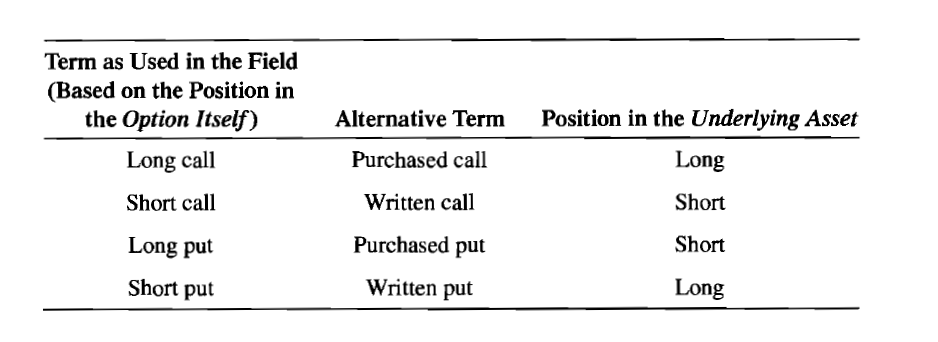
\includegraphics[scale=0.55]{picture20.PNG}

\section{Truc mnémotechnique pour les options de ventes}
POS : A \textbf{P}ut is an \textbf{O}ption to \textbf{S}ell the underlying asset.

\section{Option de vente : une assurance}
\label{sec:option vente et assurance}

Une option de vente est une assurance contre la diminution de la valeur d'un titre. Elle permet de vendre le titre à un prix prédéterminé si la valeur diminue.




%% ---------------- Chapitre 14

\chapter{Comparaison de contrats}
\label{chap:comparaison}

\section{\emph{In-the-Money} et \emph{Out-of-the-Money}}
\label{sec:in and out of the money}

Si on veut savoir la situation du \emph{payoff} à un moment \textit{t}, on le calcul selon s'il s'agit d'une option d'achat ou d'une option de vente tel que vue aux équations  : \ref{eq:chap:12:payoff long call}, \ref{eq:chap:12:payoff short call}, \ref{eq:chap:13:payoff short put}, \ref{eq:chap:13:payoff long put}.
Une terminologie est utilisé selon la valeur du \emph{payoff} :
\begin{itemize}
\item \textbf{\emph{In-the-Money option}} : La valeur du \emph{payoff} est positive.
\item \textbf{\emph{At-the-Money option}} : La valeur du \emph{payoff} est très proche de zéro (positive ou négative).
\item \textbf{\emph{Out-of-the-Money option}} : La valeur du \emph{payoff} est négative.
\end{itemize}

\section{Comparaison des positions (\emph{Long} et \emph{short})}
\label{sec:position}

Revoir le graphique à la section \ref{sec:clarification}.

\section{Comparaison des profits maximum et pertes maximales}
\label{sec:profits max et pertes max}

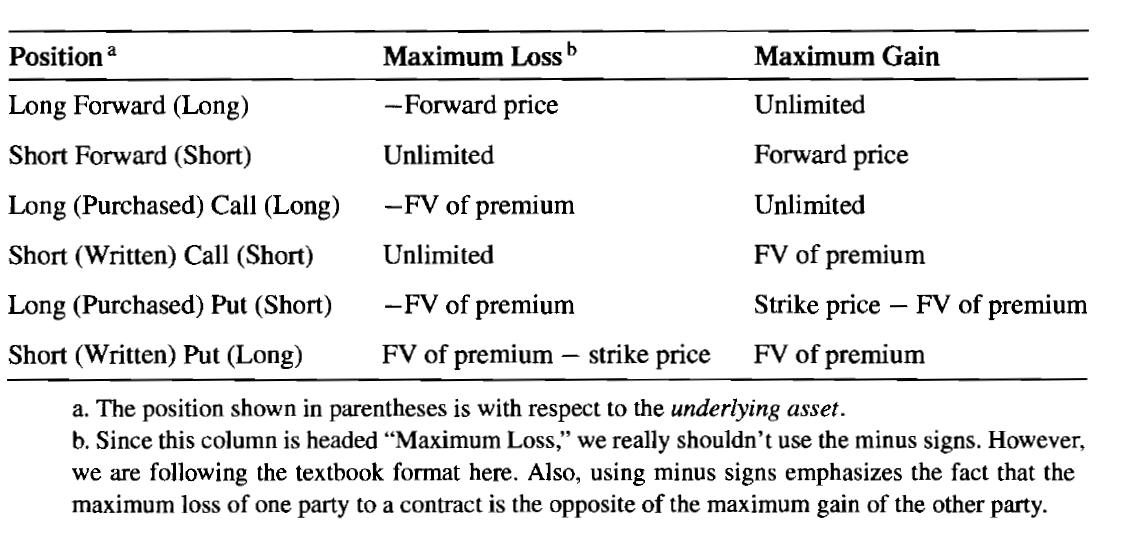
\includegraphics[scale=0.55]{picture21.PNG}

\section{Comparaison par \emph{Asset Price Contingency}}
\label{sec:asset price contingency}

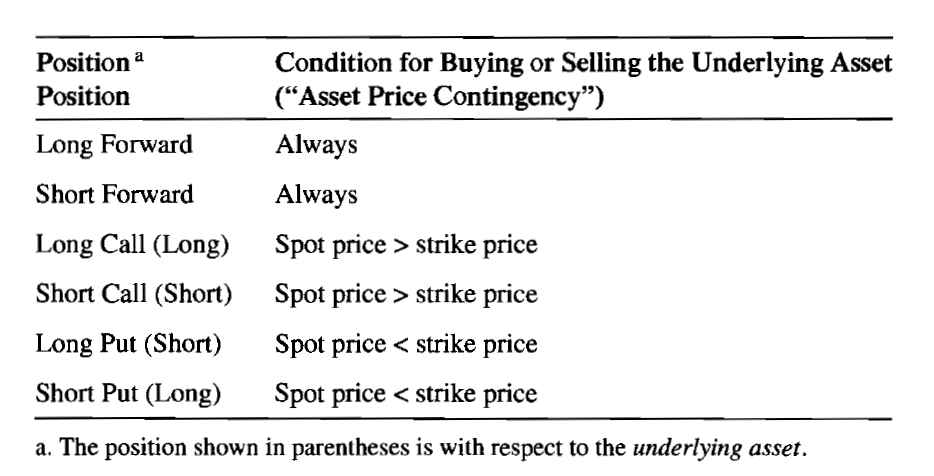
\includegraphics[scale=0.55]{picture22.PNG}

\section{Comparaison par stratégie}
\label{sec:comparaison par stratégie}

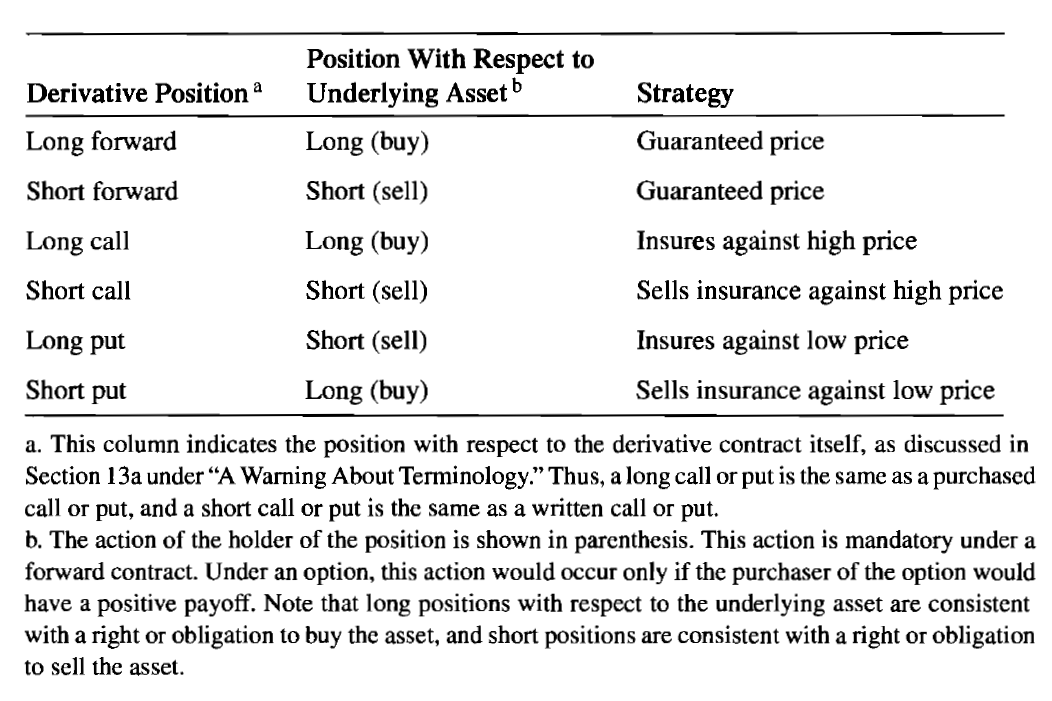
\includegraphics[scale=0.55]{picture23.PNG}

Un très bon exemple avec représentation visuel est présenté à la page 551 du document ASM.



%% ---------------- Chapitre 15

\chapter{Assuré votre position}
\label{chap:assrué position}


\section{Assuré une \emph{long position} dans un titre}

Afin de s'assurer contre la diminution de la valeur d'un titre, on peut se procurer un \emph{long put}. On appel la combinaison d'un \emph{long position} dans une action et un \emph{long put} un \emph{protective put}. La valeur minimale de \emph{payoff} dans un \emph{protective put} est la valeur du \emph{floor}. Par contre, le profit minimal du \emph{protective put} à une valeur négative correspondant à la valeur présente de la prime. 

\section{Assuré une \emph{short position} dans un titre}

Afin de s'assurer contre l'augmentation de la valeur d'un titre, on peut se procurer un \emph{long call}. La valeur maximale de \emph{payoff} est la valeur du \emph{cap/long call}. Par contre, le profit minimal du \emph{protective put} à une valeur négative correspondant à la valeur présente de la prime. Le profit reviens à un \emph{long put}.

\section{Position des \emph{writers}}

Parfois, les vendeurs d'options on des positions dans les titres. On parle alors de \emph{covered wrtiting}, \emph{option overwriting} ou de \emph{selling a covered call}. S'il ne détienne pas l'action on parle de \emph{naked writing}.

\section{Résumé des concepts}

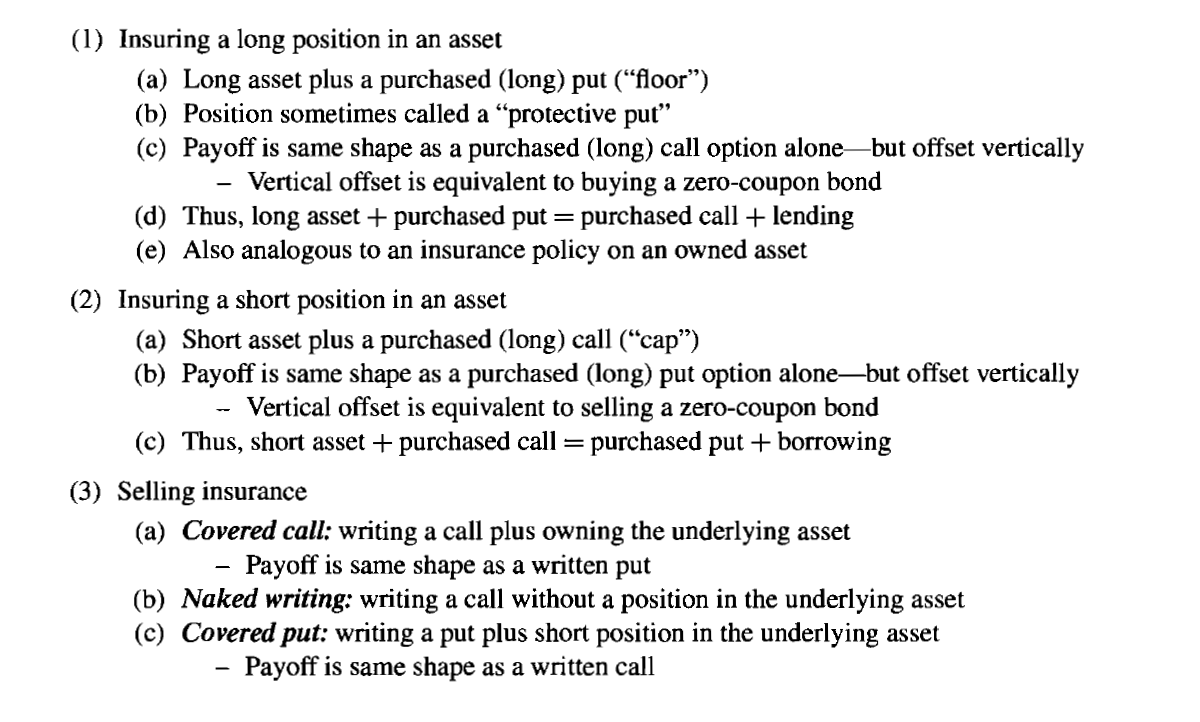
\includegraphics[scale=0.55]{picture24.PNG}



%% ---------------- Chapitre 16

\chapter{Parité \emph{put-call}, combinaison d'options}
\label{put call parity}

Vidéo d'introduction d'Investopedia : \href{http://www.investopedia.com/terms/p/putcallparity.asp?o=40186&l=dir&qsrc=999&qo=investopediaSiteSearch}{\emph{put-call parity}}.

\section{\emph{Synthetic forward contract}}
\label{sec:synthetic forward contract}

Si on combine un \emph{long call} et un \emph{short put} on obtient un \emph{synthetic long forward}. Par contre, on doit avoir le même profit, il faut donc prendre les primes en considération. Il existe des \emph{forward contrat} avec une prime appeler \emph{off-market forward} \footnote{ASM p 584-586}.

\section{Parité \emph{put-call}}


\begin{equation}
\text{Call} - \text{Put} = \text{PV(\emph{forward price})} - \text{PV(\emph{strike price})}
\end{equation}
\begin{equation}
C(K,T) - P(K,T) = PV(F_{T}) - PV(K) \Rightarrow C(K,T) - P(K,T) = PV(F_{T} - K)
\end{equation}
On peut établir la relation suivante : $ PV(F_{T}) = S_0$
Donc, 
\begin{equation}
C(K,T) - P(K,T) = S_0 - PV(K)
\end{equation}
*S'il n'y a pas de dividende.

\section{Combinaison d'options}
\label{sec:combinaison}

D'abord une révision des graphiques des différents \emph{payoff} :

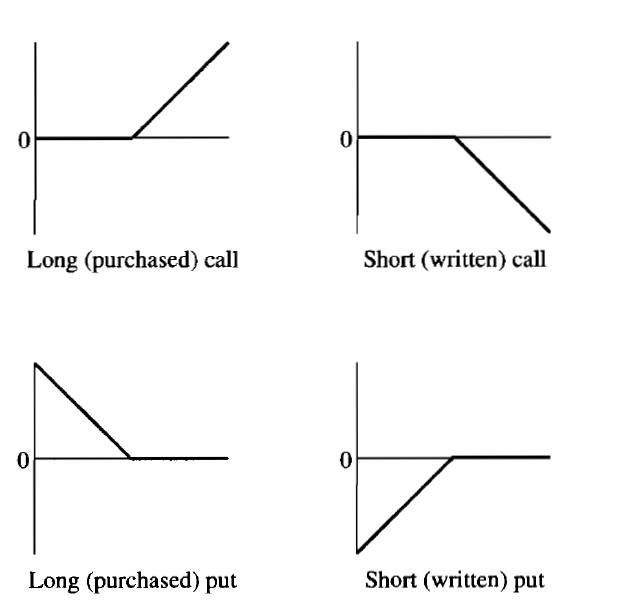
\includegraphics[scale=0.43]{picture25.PNG}

\subsection{\emph{Straddle}}
\label{sec:sec:straddle}

Définition de \emph{Straddle}: Stratégie basée sur la spéculation que le titre va être différent de ca valeur actuel. On ne favorise pas la variation dans un sens ou dans l'autre sens. Donc, un \emph{long call} et un \emph{long put} qui sont \emph{at-the-money} (\ref{sec:in and out of the money}).

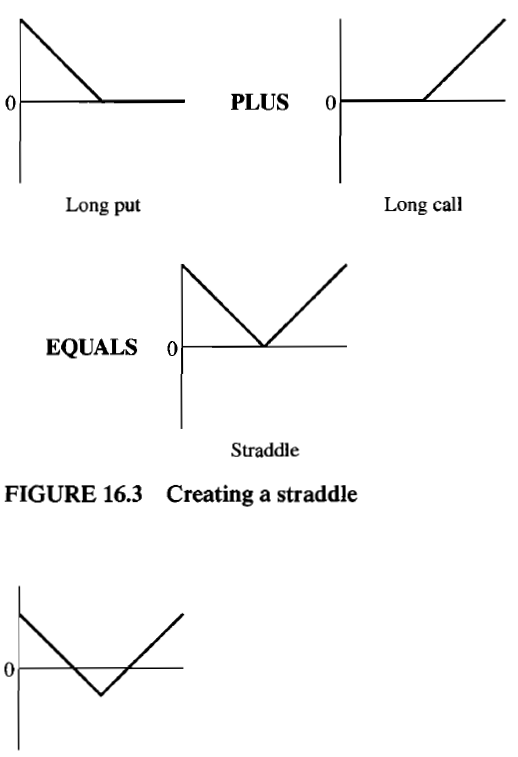
\includegraphics[scale=0.43]{picture26.PNG}

\subsection{\emph{Written/short Straddle}}
\label{sec:sec: written straddle}

Définition de \emph{Written Straddle}: Stratégie basée sur la spéculation que le titre va être très proche de ça valeur actuel. Donc, un \emph{short call} et un \emph{short put}. Il s'agit de l'opposé du \emph{Straddle} \ref{sec:sec:straddle}.

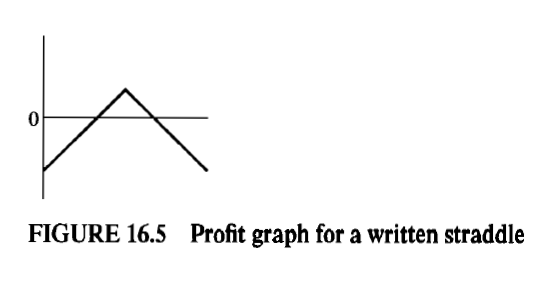
\includegraphics[scale=0.45]{picture27.PNG}

\subsection{\emph{Strangle}}
\label{sec:sec:strangle}

Définition de \emph{Strangle}: Stratégie basée sur la spéculation que le titre va être différent de ca valeur actuel. Il s'agit d'un \emph{straddle} (\ref{sec:sec:straddle}) mais avec une limitation des pertes et du rendement possible. Donc, un \emph{long call} et un \emph{long put} mais cette fois \emph{out-of-the-money} (\ref{sec:in and out of the money}).

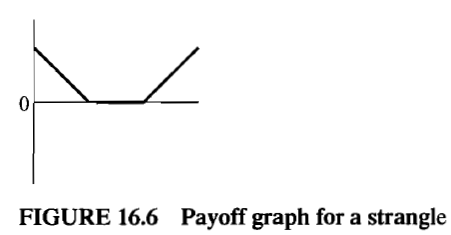
\includegraphics[scale=0.44]{picture28.PNG}
\\
Voici une comparaison des profits entre un \emph{straddle} et un \emph{Strangle} :
\\
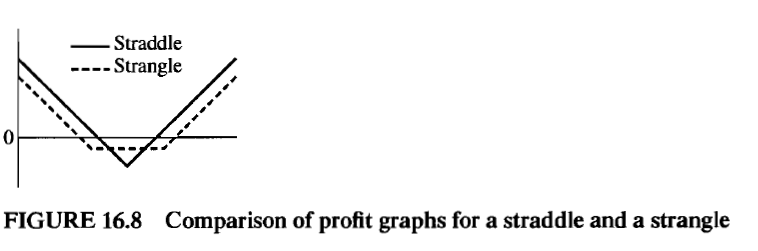
\includegraphics[scale=0.44]{picture29.PNG}

\subsection{\emph{Butterfly spread}}
\label{sec:sec:buttefly spread}

Définition de \emph{butterfly spread}: Stratégie basée sur la spéculation que le titre va être très proche de ça valeur actuel, mais en limitant les pertes contrairement à un \emph{written straddle} (\ref{sec:sec: written straddle}). Donc, un \emph{short call} et un \emph{short put} mais les deux sont \emph{out-of-the-money} (\ref{sec:in and out of the money}). On sait qu'un \emph{long call} et un \emph{short put} \emph{out-of-the-money} s'appel un \emph{strangle} (\ref{sec:sec:strangle}), donc il s'agit d'une combinaison d'un \emph{written straddle} et d'un \emph{purchased strangle}. 
\\
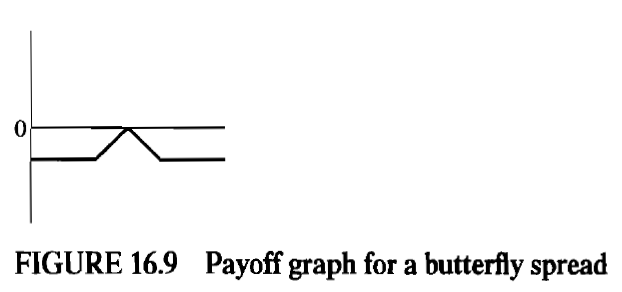
\includegraphics[scale=0.45]{picture30.PNG}


\subsection{\emph{Asymmetric butterfly spread}}
\label{sec:sec:asymmetric butterfly spread}

Similaire au \emph{butterfly spread} mais avec une forme asymétrique. L'investisseur pense donc que le prix ne varie pas beaucoup mais qu'il ne sera pas centrer. Pour construire un \emph{asymmetric butterfly spread}, on utilise une unité d'un \emph{written(short) call(K2)} avec un \emph{strike price} égale à la valeur maximale du \emph{payoff}. Ensuite deux autres options qui vont valoir le plus petit \emph{strike price(K1)} et la plus haut \emph{strike price (K3)}. Pour \textit{balancer} les deux options on utilise : $ K1 = k = \frac{K3 - K2}{K3-K1}$ et $ k3 = (1 -k)$.
\\
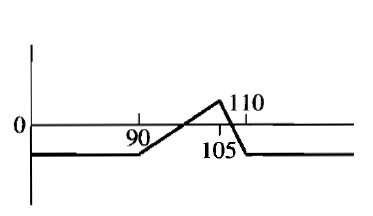
\includegraphics[scale=0.45]{picture31.PNG}

\subsection{Bull spread}
\label{sec:sec:bull spread}

Une stratégie \emph{bull} pense que le prix va monter. On utilise un \emph{long call} à un \emph{strike price} et un \emph{short call} à un \emph{strike price} plus élevé que le \emph{long call}. On peut aussi utiliser des \emph{put} avec le même système.
\\
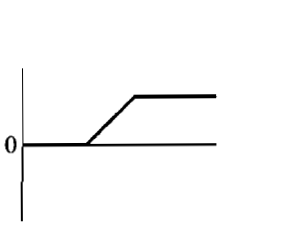
\includegraphics[scale=0.45]{picture32.PNG}

\subsubsection{\emph{Bear spread}}
\label{sec:sec:bear spread}

Une stratégie \emph{bear} pense que le prix va descendre. Opposé d'un \emph{bull spread} (\ref{sec:sec:bull spread}). On utilise un \emph{short call} à un \emph{strike price} et un \emph{long call} à un \emph{strike price} plus élevé que le \emph{long call}. On peut aussi utiliser des \emph{put} avec le même système.
\\
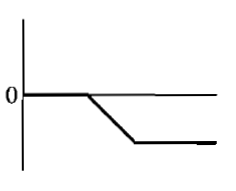
\includegraphics[scale=0.45]{picture33.PNG}

\subsection{\emph{Box spread}}
\label{sec:sec:box spread}

Cette stratégie permet d'avoir un rendement sans risque. cette stratégie est principalement utilisé lorsqu'il y a possibilité \href{http://www.investopedia.com/terms/a/arbitrage.asp?o=40186&l=dir&qsrc=999&qo=investopediaSiteSearch}{d'arbritage}. Il existe plusieurs méthodes pour obtenir un \emph{box spread} : 
\begin{enumerate}
\item \emph{synthetic long forward} (\ref{sec:synthetic forward contract} avec un \emph{strike price} de $K_1$ et un \emph{synthetic short forward} avec un \emph{strike price} plus grand que $K_1$.
\item \emph{Bull spread} de $K_1, K_2$ et un \emph{bear spread} de $K_1, K_2$.
\item \emph{Purchased strangle} de $K_1, K_2$ et un \emph{written strangle} de $K_1, K_2$.
\end{enumerate}
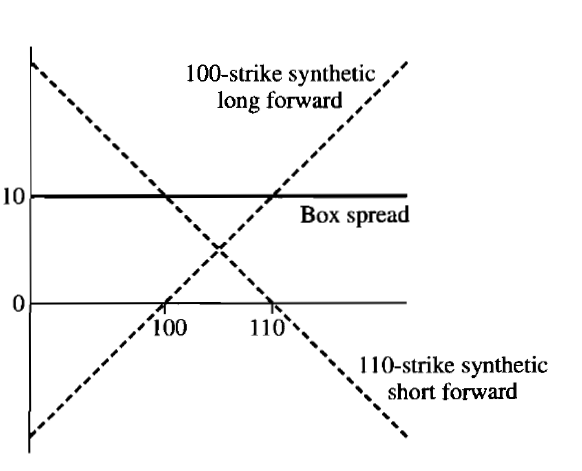
\includegraphics[scale=0.45]{picture34}

\subsection{\emph{Ratio spread}}
\label{sec:sec:ratio spread}

\emph{Ratio} signifie qu'il y a un nombre inégal de vente et d'achat d'options. La stratégie est similaire à un \emph{butterfly spread} (\ref{sec:sec:buttefly spread}) mais avec seulement une \textit{assurance} contre la diminution de la valeur.
\\
\\ 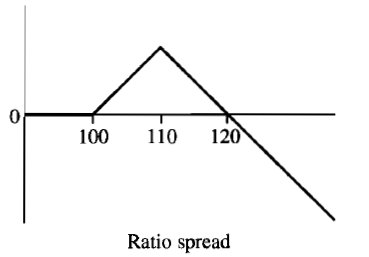
\includegraphics[scale=0.45]{picture35.PNG}

\subsection{\emph{Collar}}
\label{sec:sec:Collar}

Il s'agit d'un stratégie \emph{bear} (\ref{sec:sec:bear spread}) mais avec un payoff constant sur le \emph{collar width}). On utilise un \emph{long put} de $K_1$ et un \emph{short call} avec un \emph{strike price} plus grand que $K_1$.
\\
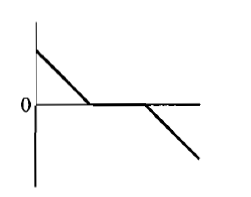
\includegraphics[scale=0.45]{picture36.PNG}

\subsubsection{\emph{Collared stock}}
\label{sec:sec:sec:collared stock}

Cette stratégie permet de se protéger contre la diminution de la valeur d'une action. On rajoute un \textit{collet} autour de l'action pour limiter les pertes et les profits. On achéte l'action et on achéte un \emph{collar} (\ref{sec:sec:Collar}). Ceci revient à faire un \emph{bull spread} avec \emph{strike price} de $K_1, K_2$.
\\
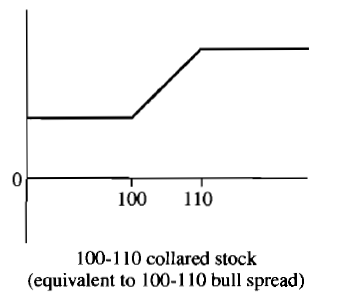
\includegraphics[scale=0.45]{picture37.PNG}
\\
Il est aussi possible de construire un \emph{zero-cost collar} (plusieurs solutions possibles).

\subsection{Résumé de la matière}
\label{sec:résumé}

Voici la feuille de formule de \href{https://drive.google.com/open?id=0B6kXivc6X9LIdkRnU09RS0VTRjA}{\textit{Coaching actuaries}}. La page 3 et 4 font une très bonne révision de la matière sur les options et les combinaisons d'options. 




%% ---------------- Chapitre 17

\chapter{Gestion de risque}
\label{chap:risk management}

Vidéo d'introduction d'\emph{Investopedia} sur le \href{http://www.investopedia.com/terms/h/hedge.asp?o=40186&l=dir&qsrc=999&qo=investopediaSiteSearch}{\emph{hedging}}.
\\ * Il s'agit de la même vidéo qu'à la section \ref{cha:produit dérivé}.
\\ On fait de la couverture d'actif pour plusieurs raisons :
\begin{enumerate}
\item Avantages fiscaux (voir exemple page 621-622)
\item Risque de faillite 
\item Méthode de financement (si proche de la faillite ou mauvais crédit)
\item Capacité de la dette (limiter l'utilisation de la dette)
\item Aversion au risque
\item Autres facteurs 
\end{enumerate}
Par contre, la couverture d'actifs nécessite des coûts direct : frais de transaction, personnel qualifié pour l'achat et la gestion ...

\section{Couverture pour le vendeur d'un titre (\emph{hedging by the seller of an asset})}
\label{sec:hedging seller}

Le vendeur d'un titre (\emph{long position}) peut chercher à se couvrir contre la dépréciation d'un titre (\emph{hedging}). Deux solution s'offre à lui:
\begin{enumerate}
\item \emph{Short forward contract} : Avec un forward contract on viens nivelé les profits à un montant constant . Varie selon les termes du contrat. (mais on bloque les profits même si la valeur du titre devient très haute)
\item \emph{Purchased put} : Viens agir à titre de valeur plancher de vente. Donc, les profits ne sont pas constant mais on viens prévenir les pertes possibles.
\end{enumerate}


\section{Couverture pour l'acheteur d'un titre (\emph{Hedging by the buyer of an asser})}
\label{sec:hedging buyer}

L'acheteur d'un titre (\emph{short position}) peut chercher à se couvrir contre l'appréciation d'un titre (\emph{hedging}). Deux solutions s'offre à lui :
\begin{enumerate}
\item \emph{Long forward contract} : Avec un forward contract on viens nivelé les profits à un montant constant . Varie selon les termes du contrat. (mais on bloque les profits même si la valeur du titre devient très basse (achat du titre))
\item \emph{Purchased call} : Viens agir à titre de valeur maximale d'achat. Donc, les profits ne sont pas constant mais on viens prévenir les pertes possibles lors de l'acaht.
\end{enumerate}

\section{Modifier la valeur de l'assurance}
On peu aussi faire varier la valeur de l'assurance de plusieurs façons :
\begin{enumerate}
\item En achetant \emph{in-the-money} (plus d'assurance) ou \emph{out-of-the-money} (moins d'assurance)
\item En rajoutant un \emph{written call} 
\item Avec un \emph{collar} (\ref{sec:sec:Collar}) (on viens \emph{cap} les profits) (on peut aussi réussir à faire un \emph{zero-cost collar})
\end{enumerate}

\section{\emph{Paylater}}
\label{sec:paylater}

Cette stratégie permet de payer une assurance seulement lorsqu'elle est nécessaire. On vend une unité d'un \emph{put} et on achète deux unités d'un \emph{put}. La prime du \emph{written put} correspond au double de la prime du \emph{purchased put}. Voir l'exemple page 626-627 pour une explication plus appronfondie.




%% ---------------- Chapitre 18

\chapter{\emph{Financial forwards and futures}}
\label{chap:forwards and futures}

\section{Comment acheter une action (4 méthodes)}

Il existe quatres méthodes pour acheter une actions :
\begin{enumerate}
\item L'acheter maintenant et la recevoir maintenant (\emph{Outright purchase})
\item L'acheter au temps \textit{t} via un contrat à terme (\emph{long forward})
\item Payer l'action maintenant et la recevoir au temps \textit{t}, un contrat à terme prépayé (\emph{prepaid forward/prepay})
\item Recevoir l'action maintenant mais payé au temps \textit{t} (\emph{fully leveraged position}) (payé $  S_0e^{rT}$ au temps \textit{t})
\end{enumerate}

\section{Prix d'un contrat à terme prépayé}
\label{sec:prepay price}

De recevoir l'action au temps 0 où au temps \emph{t} fait une différence (versement de dividende). On note un contrat à terme prépayé $ F_{0,T}^{P}$. 
\\En l'absence de dividende, on peut déterminer le prix par le principe de non-arbritage et du \emph{Market-maker} (voir page 636-637). 
\begin{equation}
F_{0,T}^{P} = S_0
\end{equation}
Avec dividende, on actualise le montant des dividendes que l'on soustrait au prix pour un \emph{outright purchase}.
\begin{equation}
F_{0,T}^{P} = S_0 - PV(dividende)
\end{equation}
Pour certain fonds négociables en bourse (\emph{ETF}, ils suivent le rendement d'un indice (DOW JONES) qui peut verser des dividendes. Étant donner la quantité des dividendes on considére qu'il s'agit d'une constante. On utilise $\delta$ mais il ne s'agit pas de la force d'intérêt, il s'agit du taux de dividende. On suppose qu'il y a réinvestissement des dividendes dans le fonds. En développent l'addition des réinvestissements on se retrouve avec $ S_t e^{\delta T}$ au temps \textit{t}. On doit dont actualisé par ce ratio $S_0$ pour obtenir le prix du contrat à terme prépayé . (voir p 638-639)
\begin{equation}
F_{0,T}^{P} = S_0e^{-\delta T}
\end{equation}

\section{\emph{Low exercise price options} (LEPO)}
\label{sec:low exercise}

Si on achete un call option pour un penny stock (action à 1 cent), on est virtuellement certain d'utilisé l'option. Le payoff ressemble à un contrat à terme prépayé. (p.639)

\section{Prix d'un contrat à terme}
\label{sec:forward contrats price}

La seule différence entre un contrat à terme et un contrat à terme prépayé est la date du paiement. Donc pour avoir le prix d'un contrat à terme on accumule au taux \textit{i} le prix d'un contrat à terme prépayé. 
Sans dividende:
\begin{equation}
F_{0,T} = S_0(1+i)^T = S_0e^{\delta T}* 
\end{equation}
* Force d'intérêt
\\Dividende discret :
\begin{equation}
F_{0,T} = S_0(1+i)^T - FV(dividendes)
\end{equation}
Dividende continu :
\begin{equation}
F_{0,T} = S_0e^{(r - \delta) T}* 
\end{equation}
Où r est le facteur d'accumulation du taux sans risque. $ (r- \delta)$ est nomé le \emph{cost of carry}) (voir document page 642)

\section{Gestion du risque pour les \emph{market-maker}}
\label{sec:risk managements market maker}

Pour gérer le risque de la transaction un \emph{market-maker} va utilisé un \emph{long forward} ou un \emph{synthetic forward} pour avoir un net \emph{payoff} de 0\$. Donc, le \emph{market-maker} fait prend une position \emph{short forward} avec le client et pour gérer son risque, il fait un \emph{long forward} ou un \emph{long synthetic forward}. Cette stratégie s'appel un \emph{cash-and-carry}. On peut aussi faire l'inverse et faire un \emph{reverse cash-and-carry}. (voir p.640-641) Résumé des stratégies :
\begin{enumerate}
\item \emph{cash-and-carry} : \emph{short forward} et acheter l'action (voir exercice 11 page 649)
\item \emph{reverse cash-and-carry} : \emph{buy forward} et \emph{short} l'action
\end{enumerate}

\section{\emph{Futures contracts}}
\label{sec:futures contracts}

Vidéo d'\emph{Investopedia} sur les \href{http://www.investopedia.com/terms/f/futurescontract.asp?o=40186&l=dir&qsrc=999&qo=investopediaSiteSearch&ap=investopedia.com}{\emph{futures contracts}}. Résumé des différences :
\\
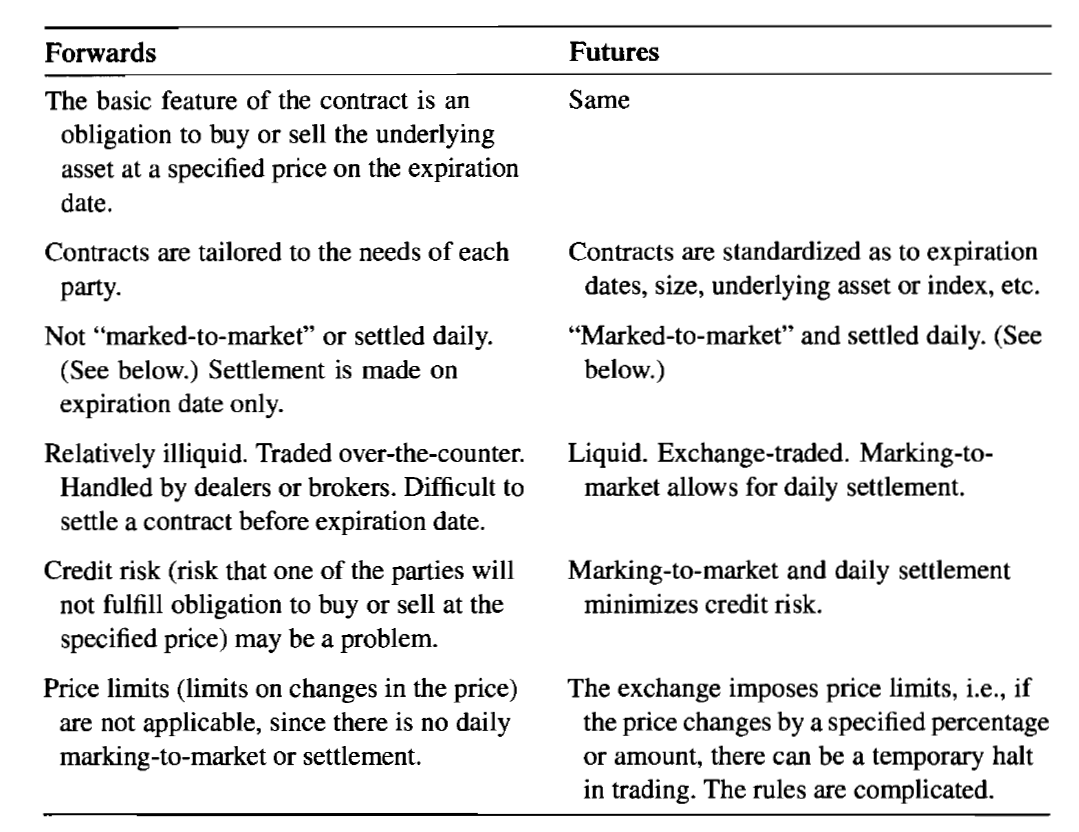
\includegraphics[scale=0.45]{picture38.PNG}
Définition de \emph{mark to market} (\href{http://www.investopedia.com/terms/m/marktomarket.asp?o=40186&l=dir&qsrc=1&qo=serpSearchTopBox&ap=investopedia.com}{vidéo}) : Il s'agit de la valeur marchande de la journée. 
\\Un \emph{future contract} nécessite un \emph{margin} pour diminuer le risque de non paiement, il y a un dépôt d'intérêt sur ce montant. (voir page 645-646)

\subsection{\emph{Quanto index contracts}}
Pour gérer le risque des contracts dans une autre devise, on utilise des contrats \emph{quanto} qui viennent éliminer le risque du taux de change. (voir page 646)




%% ---------------- Chapitre 19

\chapter{\emph{Swaps}}
\label{chap:swaps}

Un \emph{swap} est un contrat qui couvre une série de paiement sur une période. On peut donc dire qu'un \emph{forward contrat} est un \emph{swap} à paiement unique. Voici un vidéo d'\emph{Investopedia} sur le \href{http://www.investopedia.com/terms/s/swap.asp?o=40186&l=dir&qsrc=999&qo=investopediaSiteSearch}{\emph{swap}}.

\section{Règlement d'un contrat à terme}
\label{sec:règlement contrat à terme}

Différentes méthodes de règlement possibles d'un contrat à terme:
\begin{enumerate}
\item Règlement physique (échange des biens ou titres)
\item Règlement en argent
\item Règlement via un intermédiaire (\emph{brooker}) (qui fait son profit via le \emph{bid-ask spread})
\item Ràglement mixte : l'acheteur à un contrat à terme avec le \emph{brooker} et le \emph{brooker hedges} avec un second contrat à terme (pour éliminer son risque) 
\end{enumerate}

Tableaux de résumé des transactions :
\\
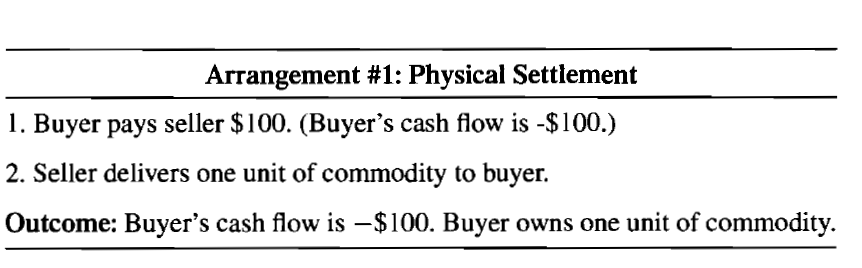
\includegraphics[scale=0.45]{picture39.PNG}
\\
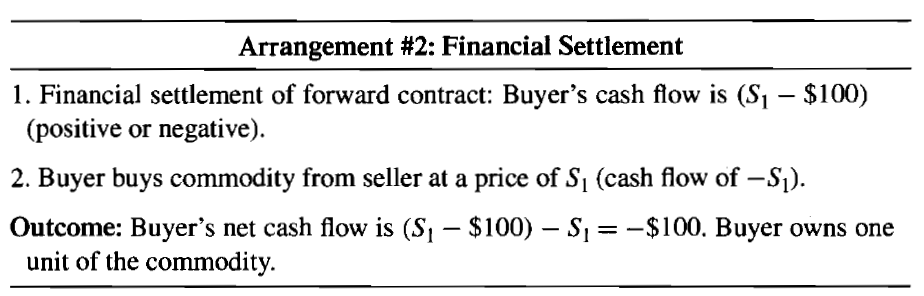
\includegraphics[scale=0.45]{picture40.PNG} 
\\
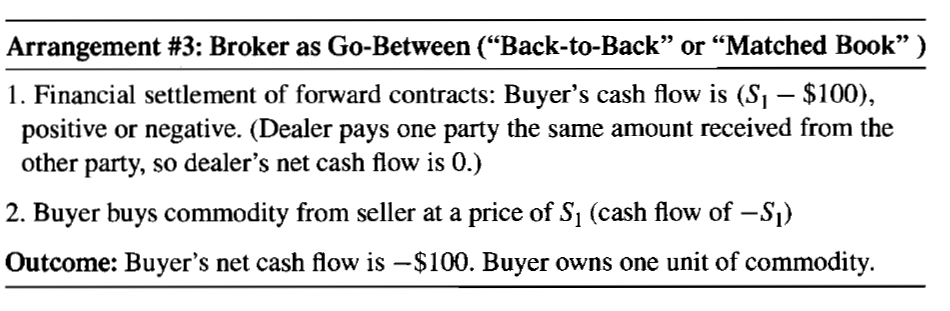
\includegraphics[scale=0.45]{picture41.PNG}
\\
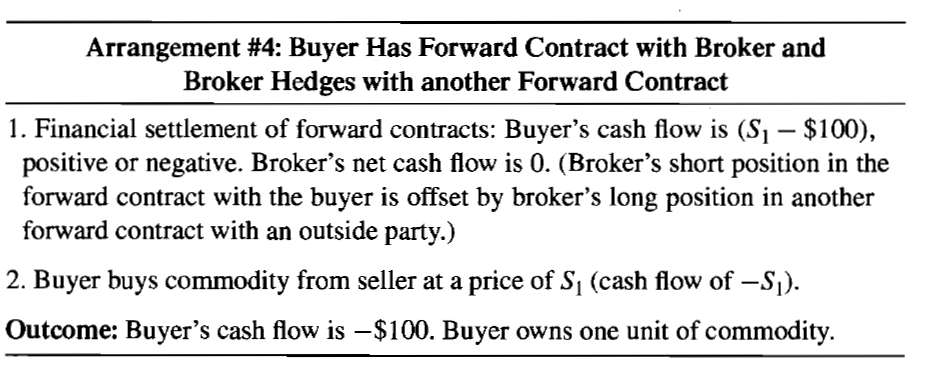
\includegraphics[scale=0.45]{picture42.PNG}

\section{Principes d'un contrat \emph{swap}}
\label{sec:swap principe}

On peut trouver le rpix d'un \emph{swap} prépayé en actualisant les prix des \emph{swap} au moments des versements. On va utilisé les taux sans risque (Spot rate \ref{sec:spot rate}) et ensuite pour facilité la gestion du risque on viens nivelé les paiements. (voir document page 655-656) À cause du nivellement, un \emph{brooker} ne peut pas totalement se protéger contre le risque à cause du risque du taux d'intérêt.

\section{Valeur marchande des \emph{swap}}
\label{swap price}

Il peut se produire deux situations : (page 658-659)
\begin{enumerate}
\item Aucun changement dans le prix des \emph{swap}
\item Il y a un changement dans le prix des \emph{swap}
\end{enumerate}

Situation 1 : La valeur marchande ne vaut pas exactement zéro parce qu'il se produit un effet de paiement en trop lors du premier versement (avec les paiements nivelés). Il y a donc une certaine valeur pour le contrat.
\\
Situation 2 : 
S'il survient un changement des prix l'acheteur peut \emph{unwind} le contrat original en entrant dans un nouveau contrat avec une \emph{short position}. La valeur du contrat créé correspond à la différence entre les paiements nivelés actualisés.

\section{\emph{Interest rate swaps}}
\label{sec:interest rate swap}

Permet de garantir le taux d'intérêt sur des prêts. Plusieurs prêts utilise des taux d'intérêts variables. Que se soit des taux d'intérêts adosser à un actifs (maison)(HELOC), taux d'intérêt suivant un indice (ARM), etc. La plupart utilise le taux de base (\emph{prime rate)}) plus un nombre de point supplémentaire. Le taux de base peut provenir de la banque centrale ou du \emph{London Interbank offer (LIBOR)}. 
\\ Pour la création d'un \emph{interest swap} voir le document 658-659. En gros, on batit avec des \emph{spot rates} un taux d'intérêt unique équivalent qui permet de nivelé. 
\\ On peut aussi vouloir un \emph{deffered swap}, on viens seulement actualisé \textit{t} périodes de plus (nombre de périodes différé). On utilise les taux \emph{forward}.
\\ Le concept s'applique aussi aux prêts avec amortissement positif (\emph{amortizing swap}) ou négatif (\emph{accreting swap}).
\\
Pour calculer un \emph{Interest rate swaps} on fait le même principe qu'un \emph{swap}. Mon taux d'intérêt \emph{forward} actualisé(avec des \emph{spot rate}) et on viens nivelé par la suite.
\begin{equation}
\frac{X}{(1+S_1)} + \frac{X}{(1+S_2)^2} + ... = \frac{\indiceGauche{1}{\vert}f}{(1+S_1)} + \frac{\indiceGauche{2}{\vert}f}{(1+S_2)^2} + ...
\end{equation}


\section{\emph{The swap curve}}
Voir document p 663-664.



%% ------------------------------------------------annexe--------------------------------------------- %%

%annexe sur la calculatrice
\appendix

\chapter{Notes supplémentaires}

\begin{enumerate}
\item Boverman offre aussi un \emph{PDF} d'explication, le document est disponible sur le \emph{Google Drive} du groupe d'échange de document dans la section du cours de \href{https://drive.google.com/open?id=0B6kXivc6X9LITmdBVFVWSDAxeE0}{mathématiques financières}.
\item J'ai mis aussi des résumés de formule du cours précédent et de la \emph{SOA} qui sont disponible dans le fichier \emph{ZIP}  \href{https://drive.google.com/open?id=0B6kXivc6X9LIYUFKaHcxNmtiUUk}{\emph{FM}}.
\item \textbf{Note sur la légende d'écriture} : 
Un symbole + signifie prochaine que la prochaine touche à \textit{cliquer} est la suivante.

\end{enumerate}

\chapter{Format d'affichage, valeur future, valeur actualisée et taux nominaux}
\label{chap:annexe affichage, futur, actualisation}


\section{Format d'affichage}
\label{sec:affichage}

\fbox{2ND} + \fbox{format} + nombre de décimale + \fbox{enter}

\section{Valeur future}
\label{sec:accumulation}

\begin{enumerate}

\item Accumulation simple
\\ (1 + taux d'intérêt) + \fbox{$ y^{x} $} + valeur de l'exposant (x) + \fbox{X} + montant à accumulé + \fbox{=}
\item Fonction TVM
\\ Légende :

\begin{enumerate}
\item \fbox{N} période ;
\item \fbox{I$ / $Y} taux d'intérêt par période ;
\item \fbox{PV} Valeur présente ;
\item \fbox{PMT} Paiement (annuité) ;
\item \fbox{FV} Valeur accumulée ;
\item Astuce : La fréquence du taux d'intérêt peut-être modifié. On pourrait mettre le taux annuel effectif et jouer avec les paramètres de la calculatrice pour avoir un taux d'intérêt mensuel.
\\ Voici comment, \fbox{I/Y} et régler à 12 pour avoir un mensuel. De base, pour ne pas faire d'erreur laisser à 1.
\end{enumerate}

\item \textbf{Comment utilisé TVM :}
\\ Nombre prériode + \fbox{N} + taux d'intérêt + \fbox{I/Y} + valeur à accumulé + \fbox{+|-} + \fbox{PV} + \fbox{CPT} + \fbox{FV}
\item \textbf{Astuce :} Pour afficher la valeur d'un des paramètres utilisé dans TVM, \fbox{RCL} + \fbox{N} ou \fbox{PV}... 
\item \textbf{Astuce :}
\begin{LARGE}
Ne pas oublier de \textit{clear} les valeurs!!
\end{LARGE}
\\ \fbox{2ND} + \fbox{CLR TVM}

\end{enumerate}

\section{Trouver le taux d'intérêt}
\label{sec:sioler i}

Nombre de période + \fbox{N} + montant à accumuler + \fbox{PV} + montant future + \fbox{FV} + \fbox{CPT} + \fbox{I/Y }

\subsubsection{Trouver i dans une annuité- cas particulier}
Dans le document ASM p. 126, à la question 8, on se retrouve avec un problème particulier. On cherche i, avec une annuité et une valeur actualisée du dernier montant. Pour résoudre ce genre de problème, il devient utile d'utilisé \textit{PV} et \textit{FV}. on affecte \textit{N} et \textit{PMT} normalement. Ensuite, on affecte la valeur présente négative de l'annuité totale et la valeur future négative du dernier paiement. 
Ex: valeur présente des paiements + \fbox{+|-} + \fbox{PV} + montant du dernier paiement + \fbox{+|-} + \fbox{FV} + \fbox{CPT} + \fbox{I/Y}

\section{Trouver le nombre de période}
\label{sec:isoler t}

Taux d'intérêt + \fbox{I$ / $Y } + valeur présente + \fbox{+|- } + \fbox{PV} + montant future + \fbox{FV} + \fbox{CPT} + \fbox{N}

\section{Taux nominal et TVM}
\label{sec:taux nominal dans TVM}

Comme les taux nominaux sont divise par le nombre de période, on peut simplement faire : \\
Nombre prériode + \fbox{N} + ($i^{(m)} \div m$) + \fbox{=} + \fbox{I/Y} + valeur à accumulé + \fbox{+|-} + \fbox{PV} + \fbox{CPT} + \fbox{FV}
\pagebreak

\section{Taux équivalent}
\label{sec:nominal to effectif}

Convertir un taux nominal en effectif : \fbox{2ND} + \fbox{ICONV} + \emph{NOM} (taux nominal) + \fbox{ENTER} + \fbox{$\Downarrow$} jusqu'à \emph{C/Y} (nombre de période) + \fbox{ENTER} + \fbox{$\Uparrow$} jusqu'à \emph{EFF} + \fbox{CPT}
\\
\\ Pour trouver un taux nominal on \fbox{CPT} \emph{NOM} et on fixe le taux effectif dans \fbox{EFF}.
\\
\\ Pour trouver un taux d'escompte, convertir \emph{d} en \emph{i}.

\chapter{Annuité et calculatrice}
\label{Annuité et calculatrice}

Pour l'utilisation de TVM, voir section \ref{sec:accumulation}, la majorité des notions de cette section sont identique pour les annuitées.

\section{Annuité due et \textit{Begin}}
\label{Begin}

La calculatrice possède une fonction \textit{Begin} qui permet de calculer l'annuité avec un paiement en début de période sans manipulation algébrique. Par contre, il faut la remettre à \textit{End} pour revenir à une annuité immédiate. Voici comment faire ;
\fbox{2ND} + \fbox{BGN} + \fbox{2ND} + \fbox{SET}.
Refaire la même procédure pour revenir à \textit{End}.

\section{Annuité à progression arithmétique}
\label{annuité et TI-30XS}
Voici une astuce pour calculer à partir des formules de la section \ref{Sub:Chap4:increasing} et \ref{Sub:Chap4:decreasing}. On utilise la calculatrice TI-30XS multiview, afin de ne pas se mélanger dans l'équation on utilise la touche \fbox{$\frac{n}{d}$}.

\chapter{Amortissement}
\label{Amortissement}

\section{TVM et fonction d'amo
rtissement}
\label{ann:chap:amortissement}
Tout d'abord, on enregistre les informations dans la fonction TVM (\textit{N}, \textit{$I/Y$}, \textit{PV}, \textit{$-$PMT}). Par la suite, \fbox{2ND} + \fbox{AMORT} + (P1) = paiement désiré + \fbox{ENTER} + \fbox{$\downarrow$} + (P2) = paiement désiré (le même) + \fbox{ENTER}, par la suite avec les fléches on peut voir le principal, la balance et l'intérêts payé. Si on veut changer de paiement on retourner à P1 et P2 pour modifier l'information\footnote{ASM p 313-314}. 
\\Note : P1 indique la ligne de début et P2 indique la ligne de fin. Donc, si P1 = 1 et P2= 3, il va s'agir du capital et de l'intérêt payé entre 1 et 3.

\chapter{Obligations}
\label{obligation}

Deux méthodes d'approche pour résoudre le prix des obligations avec la calculatrice :

\subsection{TVM et obligation}
\label{anex:TVM et obligation}

La méthode TVM :  nombre de coupons + \fbox{N} + taux d'intérêt + \fbox{I/Y} + montant du coupon + \fbox{PMT} + Valeur de rachat + \fbox{FV} + \fbox{CPT} + \fbox{PV}

\subsection{\textit{Bond worksheet}}
\label{anex:bond worksheet}

La meilleur source pour cette section est le livre d'instruction de la calculatrice voir le lien \href{https://drive.google.com/open?id=0B6kXivc6X9LIMXI4T1QtcTFQNzA}{page 65}. 

\end{document}
